%! TeX root = master.tex
% !TEX program = lualatex
\lecture{13}{19-05-2026}{Deep Learning (Part 3): NLP, RNNs and Transformers}{}

\section{From images to text}
The deep learning tools we have seen so far (MLPs, CNNs) were tailored to inputs of a
\textbf{fixed structure}: a vector of fixed size, an image of fixed resolution. \textbf{Natural
Language Processing} (NLP) breaks this assumption: a document is a sequence of words whose
length varies from sample to sample. The goals of this lecture are:
\begin{itemize}
  \item to discuss how to \textbf{represent text} (words and sequences) so it can be fed to a neural network;
  \item to introduce \textbf{recurrent neural networks} (RNNs), the historical answer to variable-length inputs;
  \item to introduce \textbf{transformers}, the architecture that has come to dominate modern NLP (and beyond).
\end{itemize}

\section{Representing text}
\subsection{The heterogeneity problem}
Text data is naturally \textbf{heterogeneous in length}: documents in the 20~Newsgroups
dataset, for instance, range from a one-line apology to a long technical post. For supervised
methods like an MLP or a softmax classifier, we have always assumed inputs of identical size,
so we need a way to turn an arbitrary piece of text into a fixed-size representation, or to
build models that natively accept variable-length sequences.

\subsection{Bag of Words: a document-level representation}
A first idea is the \textbf{Bag of Words (BoW)} representation seen earlier in the course:
fix a dictionary of $D$ words and represent each document by a vector
$\tilde{\mathbf{x}} \in \mathbb{R}^{D}$ where entry $i$ counts how many times the $i$-th word
appears in the document. Two documents are then compared by comparing their word
\emph{counts}.

BoW is fine when the task is at the \textbf{document level} (sentiment analysis, author age
prediction, topic classification), but it has two strong limitations:
\begin{itemize}
  \item it \textbf{throws away word order} -- ``the dog bit the man'' and ``the man bit the dog'' look identical;
  \item it cannot solve \textbf{word-level tasks} such as named entity recognition, translation, or text generation, where we need a representation for each individual word.
\end{itemize}
This motivates moving from document-level to \textbf{word-level} representations.
\clearpage
\subsection{Word representations}
How do we represent natural language sequences for NLP problems ? 

\begin{center}
Sentiment analysis problem

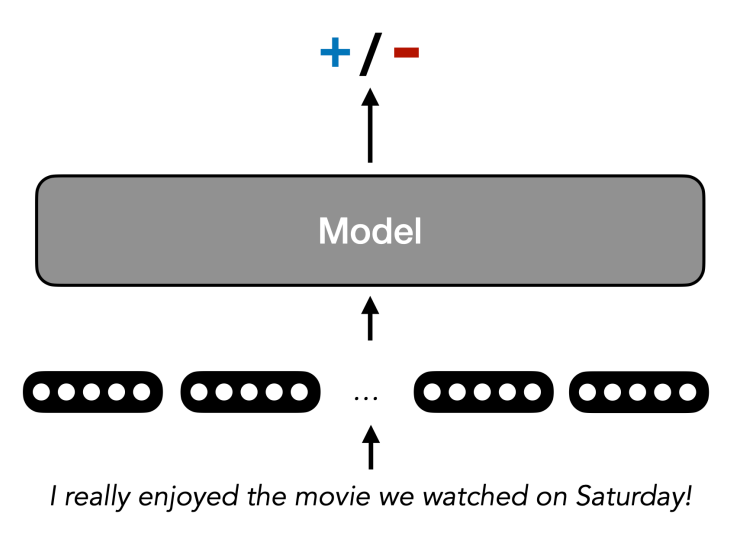
\includegraphics[width=0.4\linewidth]{images/img_20260519_101839.png}
\end{center}

The way neural language processing (NLP) do it is by representing \textbf{words} as \textbf{vectors}, thus a sentence becomes a sequence of vectors. 

\subsection{Words as vectors: the naive one-hot approach}
The simplest way to represent each word as a vector is to assign each word a unique index in
a vocabulary $V$ and use a \textbf{one-hot vector} $x_i \in \{0, 1\}^{|V|}$: every entry is $0$
except the one corresponding to the word, which is $1$.

\begin{center}
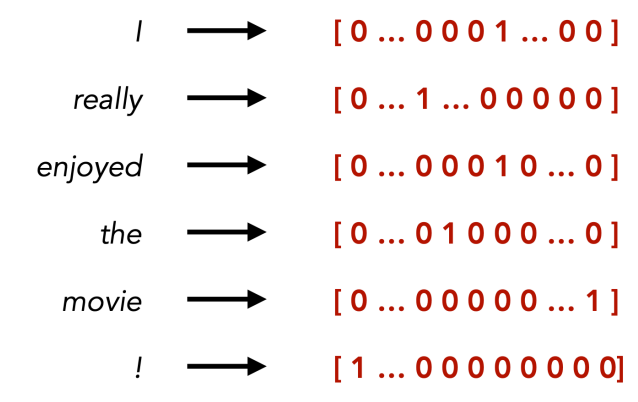
\includegraphics[width=0.4\linewidth]{images/img_20260519_100916.png}
\end{center}

But this representation has two serious drawbacks:
\begin{itemize}
  \item \textbf{Huge dimensionality}: vocabularies easily reach $10^4$--$10^6$ words.
  \item \textbf{No notion of similarity}: any two distinct words are \emph{orthogonal}.
        For example, \emph{enjoyed} and \emph{loved} are semantically very close yet their
        one-hot vectors have cosine similarity $0$. The model would have to relearn the
        meaning of each word independently from data.
\end{itemize}

\subsection{Word embeddings}
\textbf{Word embeddings} replace the sparse one-hot vector with a \textbf{high-dimensional, real-valued}
vector in $\mathbb{R}^{d}$, with $d$ typically in $O(10^{2}$--$10^{3})$ -- still much smaller
than $|V|$. The crucial property is that:
\begin{center}
  \emph{the geometry of the embedding space reflects the semantics of words.}
\end{center}
Words with similar meaning end up close together, and even directions in the embedding space
become meaningful. 
\begin{center}
   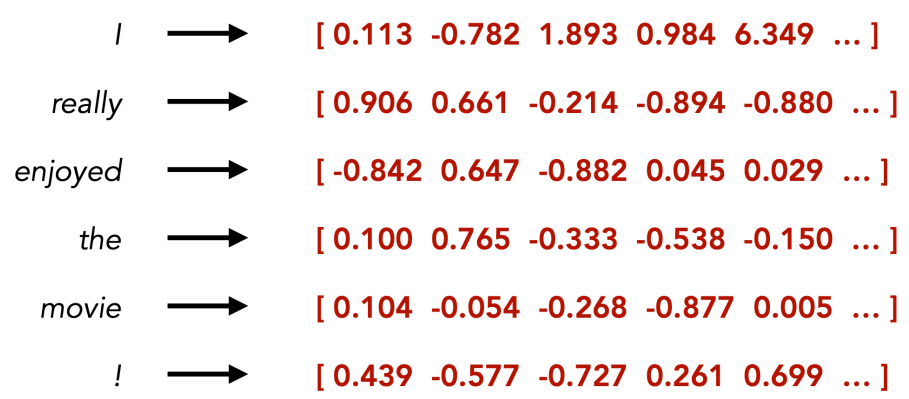
\includegraphics[width=0.5\linewidth]{images/img_20260519_102120.png}
\end{center}

\paragraph{Example}
In those illustrations we see that words with similar meaning are close. 
And crazier that for example $\text{king} - \text{man} + \text{woman} \approx \text{queen}$, and that the direction going
from a country to its capital is roughly constant across country/capital pairs.
\begin{center}
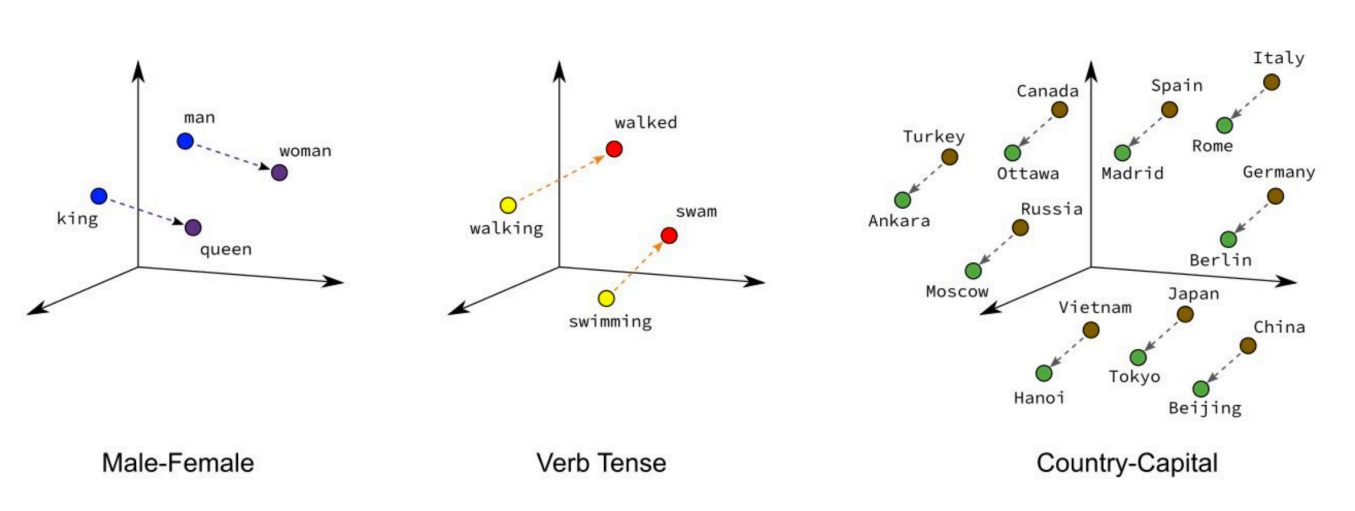
\includegraphics[width=\linewidth]{images/img_20260519_102244.png}
\end{center}

\paragraph{The dot product measures alignment}
Because words now live in $\mathbb{R}^{d}$, comparing two words means comparing two vectors,
and the natural tool is the \textbf{dot product}. Geometrically it tells us how well two
vectors \emph{align}: it is positive when they point in similar directions, zero when they are
perpendicular, and negative when they point in opposite directions. Computationally it is just
a weighted sum of coordinates -- exactly the kind of operation deep networks are built from.

This also lets us \emph{quantify} a semantic direction. Suppose we conjecture that
$\text{cats} - \text{cat}$ encodes a ``plurality'' direction. Taking the dot product of this
vector with singular nouns and with their plurals, the plurals consistently score higher;
dotting it against the embeddings of \emph{one, two, three}, \dots\ even gives increasing
values. A direction in the space thus carries meaning, and the dot product measures how
strongly a word expresses it -- the very operation the attention scores will rely on.

\subsubsection{How are embeddings learned?}
Two paradigms exist:
\begin{itemize}
  \item \textbf{Supervised}: optimize the embeddings for a specified task (e.g, sentiment analysis). 
    This works but requires labels and the
        learned embeddings are \emph{task-specific} -- they may not generalize to other tasks.
  \item \textbf{Unsupervised (or self-supervised)}: learn embeddings from raw, unlabelled text by exploiting
        the structure of language. The guiding principle is Firth's quote (1957):
        \begin{quote}\centering ``You shall know a word by the company it keeps.''\end{quote}
        Concretely, the meaning of a word is approximated by looking at the words that
        typically appear \textbf{nearby}. For example, the blank in ``\emph{I really enjoyed
        the \rule{0.6cm}{0.4pt} we watched on Saturday}'' is very probably \emph{movie} or
        \emph{game}, and the corresponding embeddings should be similar.
\end{itemize}
\textbf{Word2Vec} and \textbf{GloVe} are the standard self-supervised approaches that exploit
this idea.

\textbf{Remark.} Word embeddings are pre-trained once on a huge corpus and then \emph{reused}
as a fixed lookup table for downstream tasks -- a first form of \emph{transfer learning} 
(a machine learning technique where a model pre-trained on a large dataset is reused as the starting point for a new, related task) in NLP.

\subsection{Why individual words are not enough}
Even with great word embeddings, processing words \textbf{one at a time} is unsatisfactory:
\begin{itemize}
  \item we still face the \textbf{heterogeneity} problem -- documents have variable length;
  \item individual words can be \textbf{misleading}: in the review
        \emph{``The restaurant refused to serve me a ham sandwich, because it only cooks
        vegetarian food. \dots Their ambience was just as} \textbf{good} \emph{as the food
        and service.''}, the word \emph{good} is positive in isolation but the surrounding
        context determines whether the review is actually a praise or a complaint.
\end{itemize}
Therefore, instead of modeling words, we want to model a complete sentence or document as a sequence.

Note that each individual word is still modeled as a vector as discussed previously.

\paragraph{Embeddings that soak up context}
In that very first step, each vector is simply plucked out of the embedding table, so it can
only encode the meaning of a \emph{single word in isolation}, blind to its neighbours. The
whole purpose of the network that follows is to let each vector progressively \textbf{absorb
context}, so that by the end it points in a far more specific direction. A vector that starts
its life as the embedding of \emph{king}, for instance, can be gradually tugged by the
successive blocks until it encodes ``a king who reigned in Scotland, who seized the throne by
murdering his predecessor, and is described in Shakespearean English'' -- i.e.\ \emph{Macbeth}.
The token is unchanged; its meaning has been enriched by everything around it. This contextual
enrichment is precisely the job of the \textbf{self-attention} mechanism introduced next.
\section{Modeling sequences}
\subsection{Sequence-to-sequence: encoder--decoder}
The dominant template for such models is the \textbf{encoder--decoder} (also called
\textbf{sequence-to-sequence}, or seq2seq) architecture. The \textbf{encoder} reads the input
sequence and compresses it into a representation; the \textbf{decoder} produces an output
sequence from this representation. 
\vspace{-8pt}
\paragraph{Example} 
Translation: 
an encoder reads a French sentence and a decoder writes the English translation.
\begin{center}
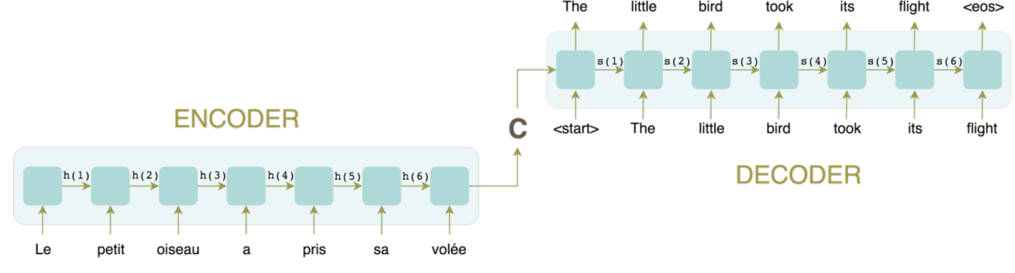
\includegraphics[width=0.9\linewidth]{images/img_20260519_114647.png}
\end{center}

The remaining question is: \emph{how do we model each of these blocks?} Historically, the
answer was \textbf{recurrent neural networks}; today it is \textbf{transformers}. But let's see how they both work.

\section{Recurrent Neural Networks (RNNs)}
\subsection{Idea}
A \textbf{Recurrent Neural Network} is a neural network with a \textbf{feedback loop}: it
maintains an internal \textbf{state} $h_t$ that is updated at each time step from the new
input $x_t$ and the previous state $h_{t-1}$. The state then summarizes everything seen so
far.
\begin{center}
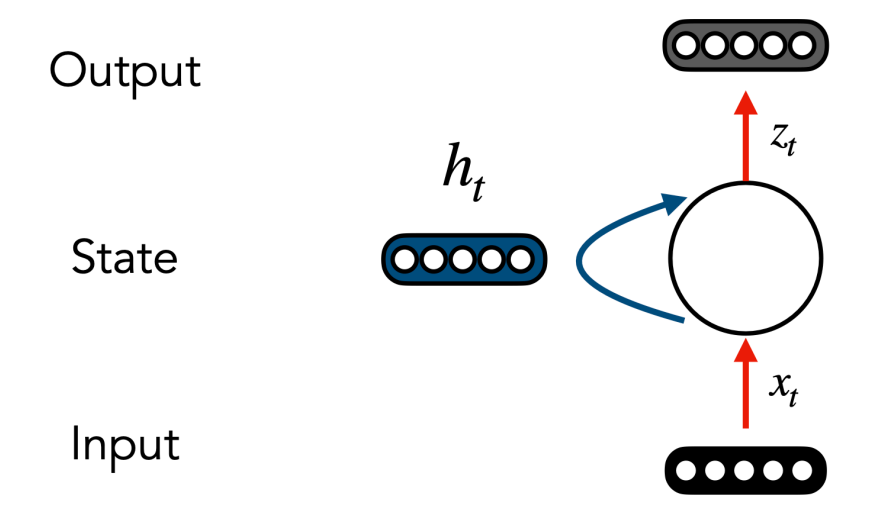
\includegraphics[width=0.4\linewidth]{images/img_20260519_132504.png}
\end{center}

\subsection{Unrolling}
The recurrence is conceptually a loop, but for computation and visualization we
\textbf{unroll} the network across time, obtaining a feed-forward graph where each time step
has its own cell sharing the \emph{same} weights:
\begin{center}
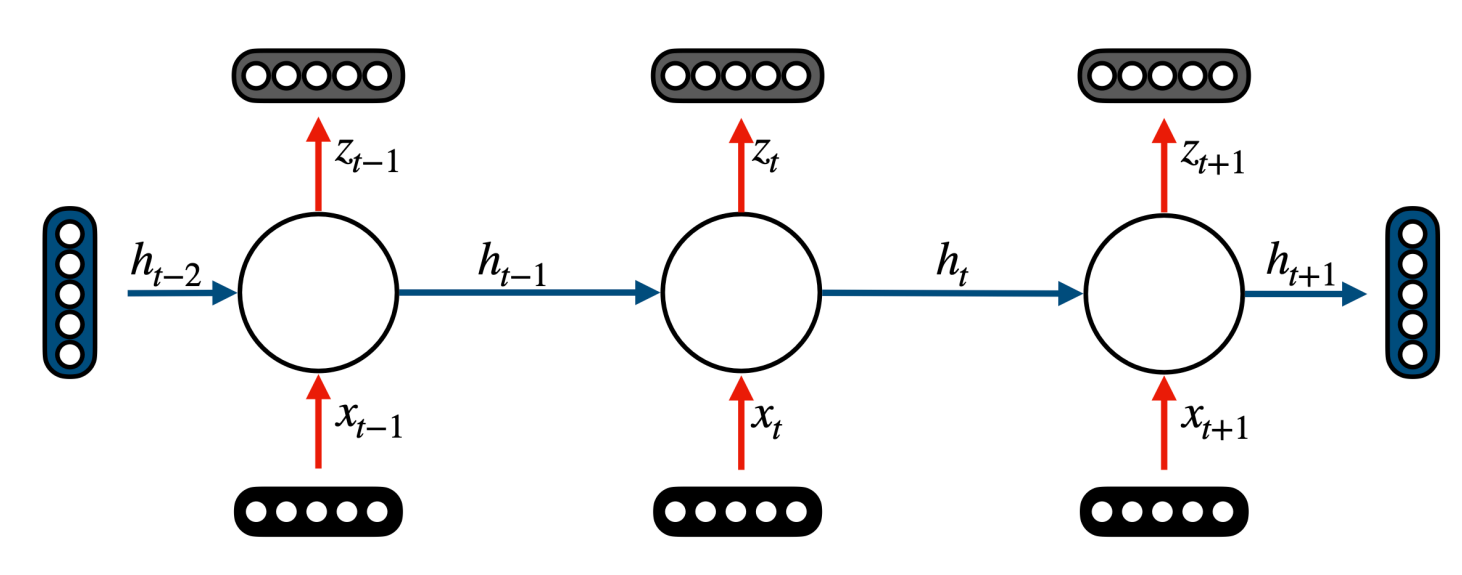
\includegraphics[width=0.7\linewidth]{images/img_20260519_132555.png}
\end{center}

\textbf{Crucially, the same parameters are reused at every time step.} This makes the model
applicable to sequences of \emph{any length}, regardless of what was seen at training time.
\vspace{-8pt}
\paragraph{Example} Making a sentence of 5 words : \textit{"The starving cat fanatically chased"}, results to updating the internal state 5 times
\begin{center}
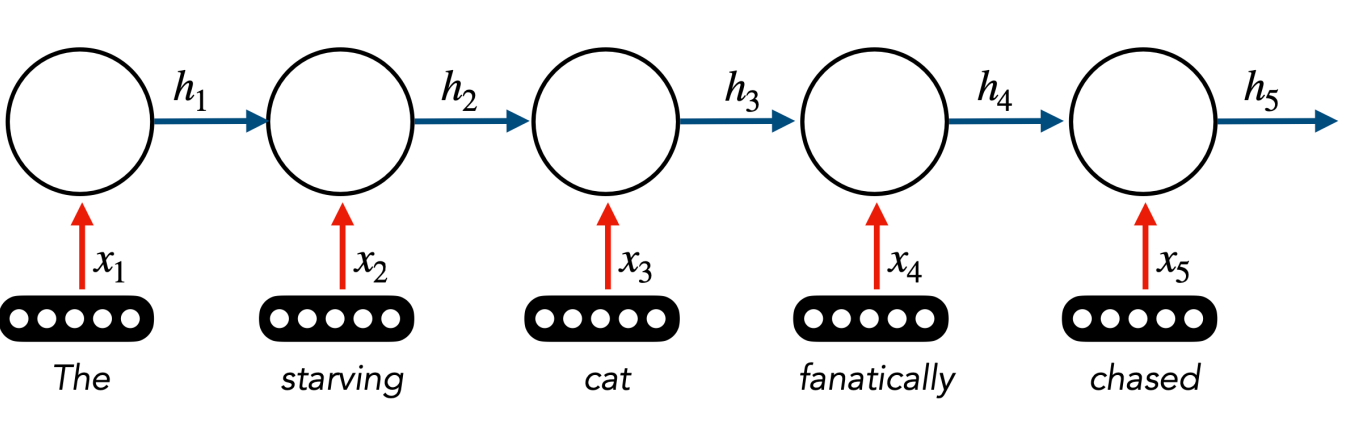
\includegraphics[width=0.7\linewidth]{images/img_20260519_133310.png}
\end{center}


\subsection{Equations for the standard (Elman) RNN}
For an input sequence $\{x_t\}$, the basic RNN computes
\[
  h_t = \sigma\big( W_{hx}\, x_t + W_{hh}\, h_{t-1} + b_h \big), \qquad
  z_t = \sigma\big( W_{zh}\, h_t + b_z \big),
\]
where $\sigma$ is a non-linear activation (often $\tanh$), $h_t$ is the hidden state and
$z_t$ is the output at time $t$. The weight matrix $W_{hx}$ transforms the input $x_t$ so he could contribute to the new state (same for $W_{hh}$), $W_{zh}$ is the matrix that project the hidden state to the output space.
We could see the matrix as traductors, from a space to an other. All three weight matrices and the two biases are
\emph{shared} across time steps.

\subsection{Three uses of an RNN}
Depending on what we read off the unrolled network, an RNN can be used for very different
tasks.

\subsubsection{Sequence classification}
We feed the whole sequence to the RNN and use only the \emph{last} output $z_T$ as a summary,
which is fed to a classifier (a linear projection followed by a sigmoid for binary tasks or
a softmax for multi-class):
\[
  \textbf{Binary: } P(y) = \sigma(W_o z_T) \qquad \textbf{Multi-class: } P(y) = \mathrm{softmax}(W_o\, z_T).
\]
This is what one would do for, e.g, sentiment analysis.
\begin{center}
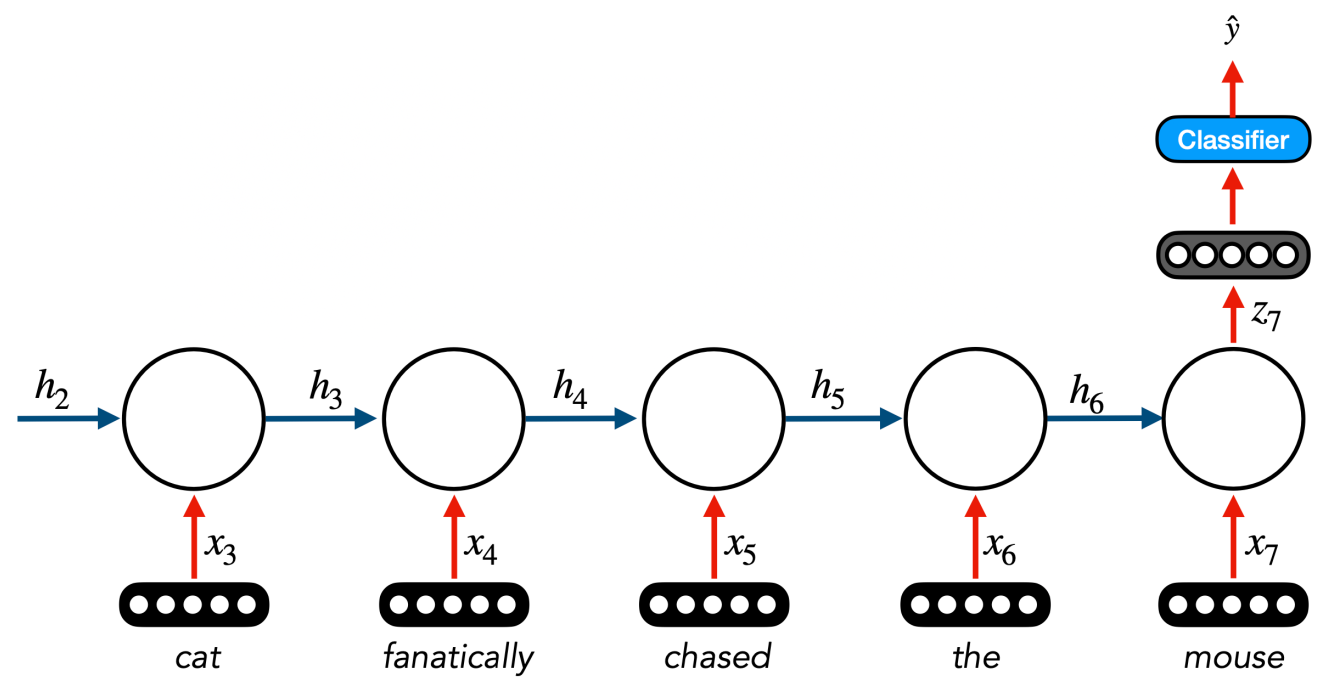
\includegraphics[width=0.7\linewidth]{images/img_20260519_134704.png}
\end{center}

\subsubsection{Sequence labeling}
For per-word tasks (e.g, part-of-speech tagging, named entity recognition), we attach a
classifier to \emph{every} output $z_t$ to produce one label per token.

\begin{center}
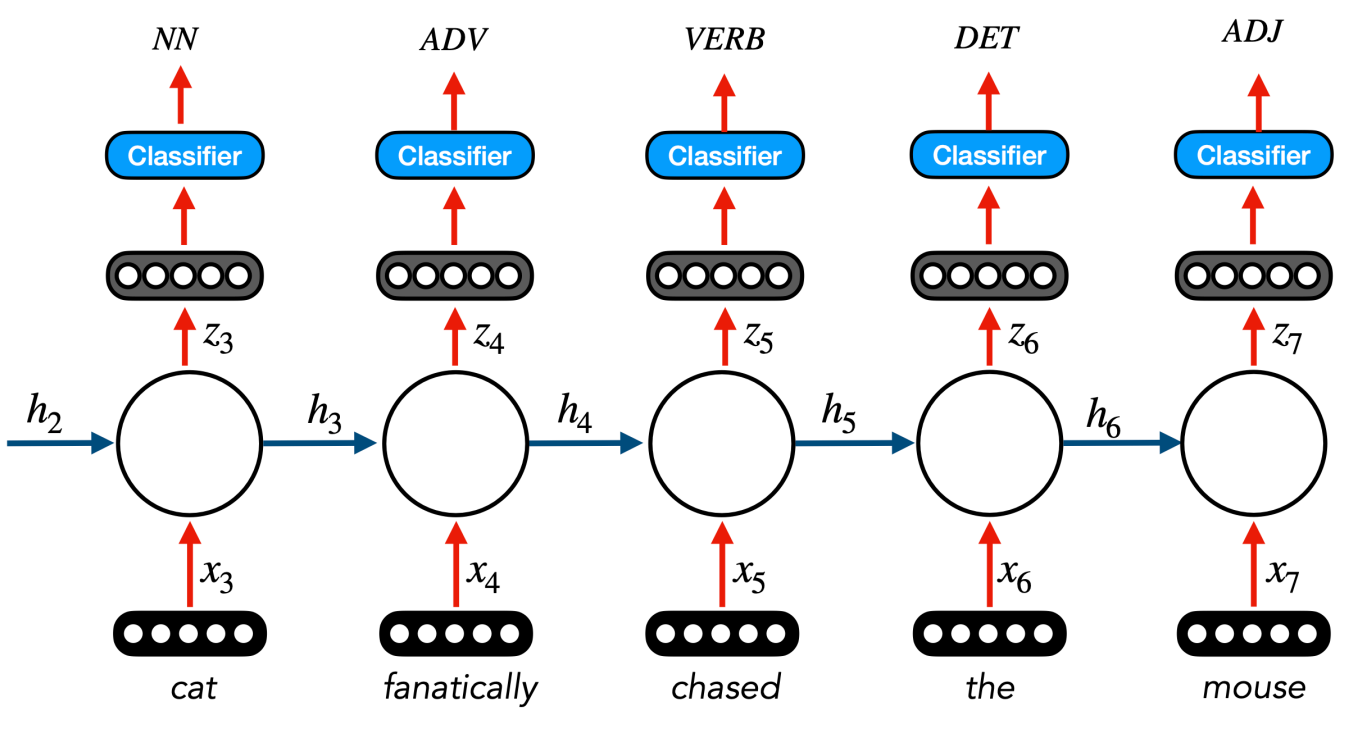
\includegraphics[width=0.7\linewidth]{images/img_20260519_135226.png}
\end{center}

\subsubsection{Generation}
To \textbf{generate} text, we feed the predicted output of step $t$ as the input of step
$t+1$. Starting from a special start token (and possibly some context), the RNN produces a
sequence one token at a time until it emits an end-of-sequence (\texttt{<EOS>}) token.

\begin{center}
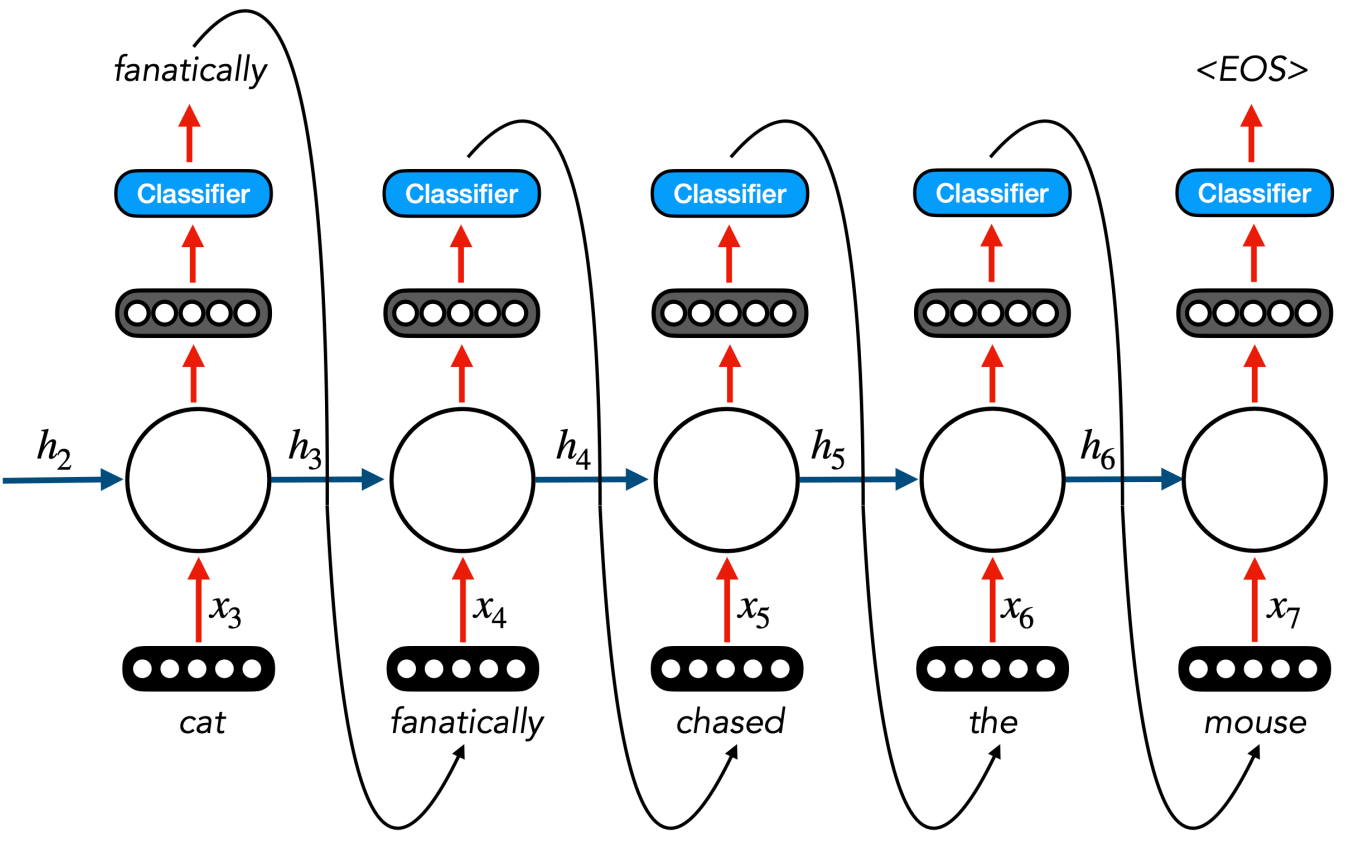
\includegraphics[width=0.7\linewidth]{images/img_20260519_135427.png}
\end{center}

\subsection{RNN variants: LSTM and GRU}
The standard RNN above struggles to remember information across many time steps -- when we
backpropagate through many copies of the same weights, gradients tend to vanish (or explode).
This issue was already encountered in deep MLPs, and is more severe here because the depth is
the length of the sequence.

Two improved cells are commonly used in practice:
\begin{itemize}
  \item \textbf{LSTM} (Long Short-Term Memory): introduces a
        separate \textbf{cell state} $c_t$ and three \emph{gates} (input, forget, output) that
        control what is written to, read from, and erased from the cell. The gates use
        sigmoids and elementwise products, allowing the network to learn to keep information
        for many steps.
  \item \textbf{GRU} (Gated Recurrent Unit): a simplified gated cell with
        only two gates (update, reset). Cheaper than an LSTM, comparable performance in many
        applications.
\end{itemize}
\begin{center}
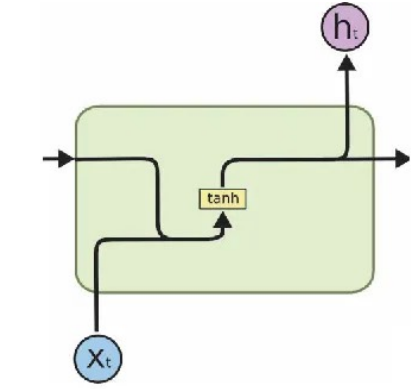
\includegraphics[width=0.22\linewidth]{images/img_20260519_135819.png}
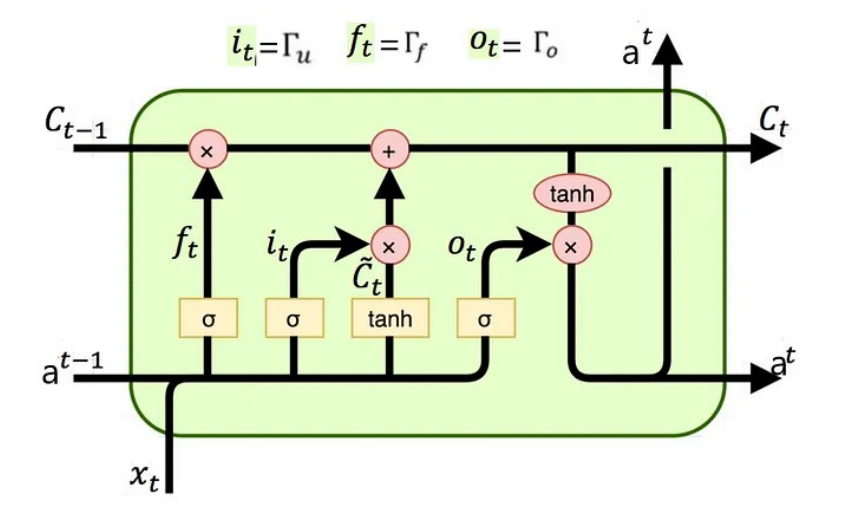
\includegraphics[width=0.3\linewidth]{images/img_20260519_135753.png}
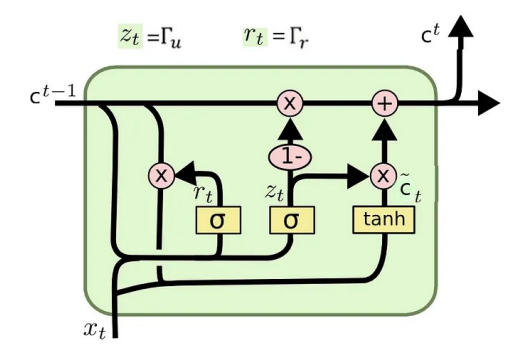
\includegraphics[width=0.29\linewidth]{images/img_20260519_135829.png}
\end{center}

\textbf{Remark.} For the purposes of this course, the important point is that an LSTM (or
GRU) is just an RNN with a more careful internal cell that mitigates vanishing gradients
and learns longer-range dependencies. The high-level behaviour -- a recurrent cell processing
a sequence one token at a time -- is exactly the same.

\subsection{Training an encoder--decoder RNN}
For an encoder--decoder model, both the encoder and the decoder are RNNs (typically LSTMs).
The encoder processes the input sequence; its final hidden state initializes the decoder, which
generates the output sequence token by token. The model is trained by minimizing the
\textbf{average cross-entropy} of the predicted tokens with respect to the ground-truth output:
\[
  \mathcal{L} \;=\; \sum_{t=1}^{T} -\log P\big( y_t \;|\; y_1, \dots, y_{t-1},\; x_1, \dots, x_n \big).
\]
Gradients are backpropagated through both the decoder and the encoder.

\begin{center}
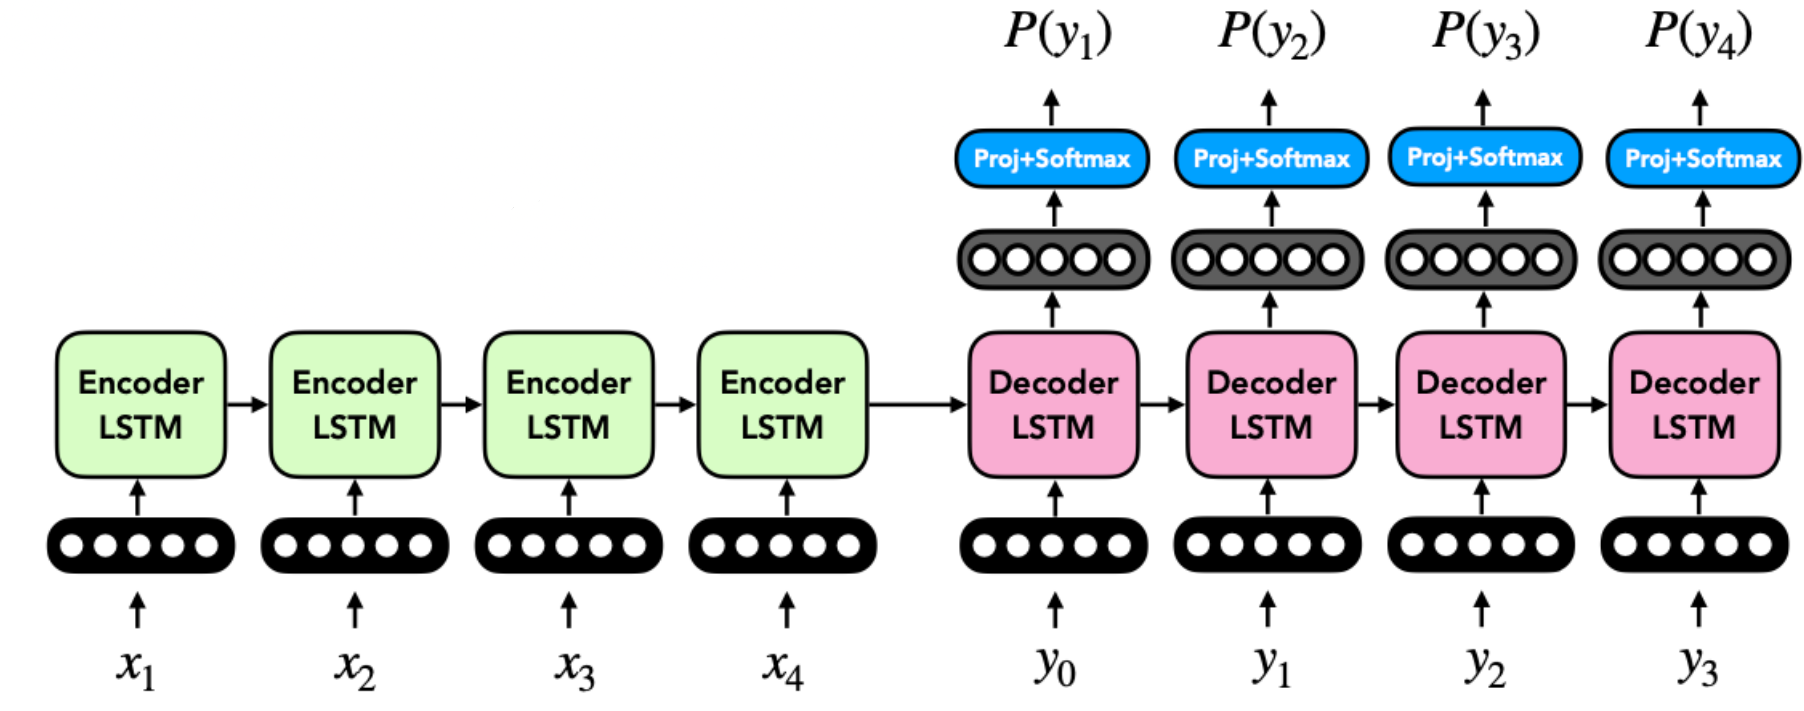
\includegraphics[width=0.8\linewidth]{images/img_20260519_140300.png}
\end{center}

\subsection{Limitations of RNNs}
RNNs suffer from two structural problems:
\begin{itemize}
  \item the \textbf{state is a single fixed-size vector}, thus it is a massive compression of information.
  \item it is \textbf{hard to learn long-range dependencies}, despite LSTMs/GRUs, especially
        when the relevant information is many steps away from where it is needed.
\end{itemize}

\section{Attention}
\subsection{Motivation}
The RNN encoder produces a hidden state $h_t^{e}$ at \emph{every} time step, not just at the
end. Instead of throwing all of these away and keeping only the last one, the
\textbf{attention mechanism} lets the decoder, at each generation
step, look back at \emph{all} encoder states and decide which ones are relevant. The decoder
\emph{focuses on different parts of the input at different generation steps}.
\begin{center}
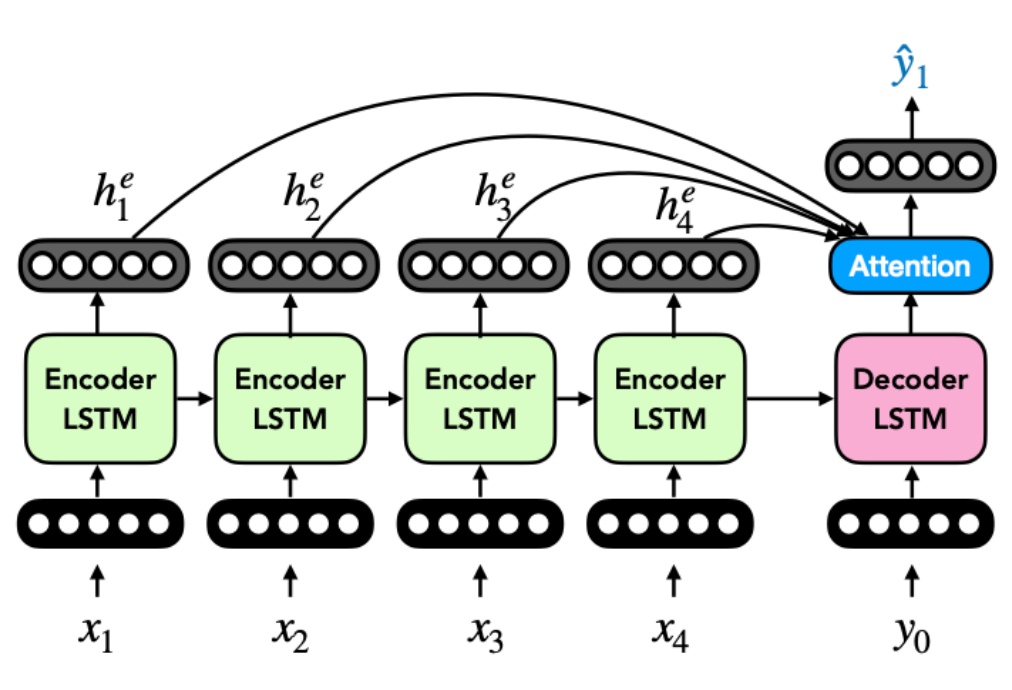
\includegraphics[width=0.5\linewidth]{images/img_20260519_142132.png}
\end{center}

\subsection{The attention function}
At decoding step $1$, the current decoder hidden state $h^{d}_{1}$ is compared with each
encoder hidden state $h^{e}_t$ via a \emph{similarity function} $f$, producing a raw
\textbf{attention score} ("idea of what to decode"):
\[
  a_t = f\big( h^{e}_{t},\, h^{d}_{1} \big), \qquad t = 1, \dots, T.
\]
Three classical choices for $f$ are summarised below:
\begin{center}
\begin{tabular}{ll}
\hline
\textbf{Attention Function} & \textbf{Formula} \\
\hline
Multiplicative   & $a = h^{e}\, \mathbf{W}\, h^{d}$ \\
Linear           & $a = v^{T}\, \phi\!\left( \mathbf{W}\,[h^{e};\, h^{d}] \right)$ \\
Scaled dot prod. & $a = \dfrac{(\mathbf{W} h^{e})^{T}\,(\mathbf{U} h^{d})}{\sqrt{d}}$ \\
\hline
\end{tabular}
\end{center}
The scaled dot product is what transformers use; the scaling by $\sqrt{d}$ keeps the
magnitude of the dot product bounded as the dimension $d$ grows, which stabilises training.

The raw scores are then turned into a \textbf{probability distribution} over the encoder
states via softmax:
\[
  \alpha_t \;=\; \frac{e^{a_t}}{\sum_{j} e^{a_j}},
\]
and the resulting \textbf{context vector} is a weighted average of the encoder states:
\[
  \tilde{h}^{d}_{1} \;=\; \sum_{t=1}^{T} \alpha_t\, h^{e}_{t}.
\]

\begin{center}
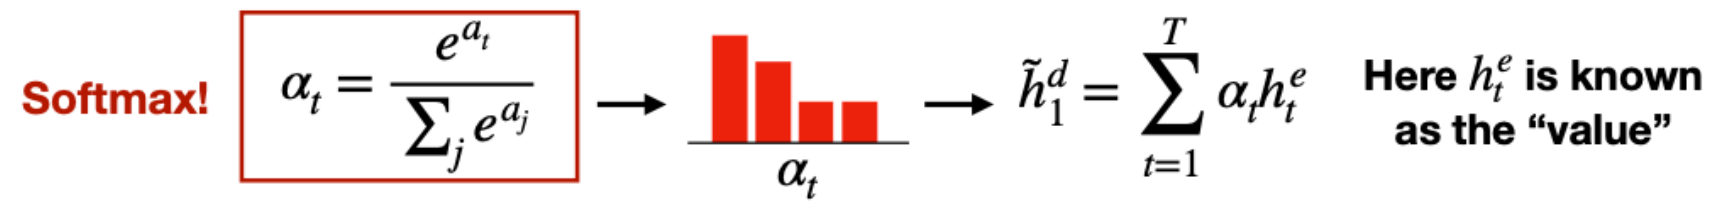
\includegraphics[width=0.8\linewidth]{images/img_20260519_143220.png}
\end{center}

\textbf{Terminology to remember.} In this picture:
\begin{itemize}
  \item the decoder state $h^{d}$ that we use to ``ask the question'' is the \textbf{query};
  \item each encoder state $h^{e}_{t}$ plays two roles:
        \begin{itemize}
          \item as a \textbf{key}, against which the query is compared (computes $a_t$) "answering the question";
          \item as a \textbf{value}, which is the thing being summed in the weighted average.
        \end{itemize}
\end{itemize}
This query/key/value vocabulary will become essential when we describe self-attention.

\subsection{The attentive encoder--decoder}
Once $\tilde{h}^{d}_{1}$ has been computed, it is \textbf{concatenated} (or otherwise
combined) with the original decoder state $h^{d}_{1}$, and fed to the output layer to predict
the most likely token $\hat{y}_{1}$. The decoder then advances to the next step, recomputes a
new attention distribution from $h^{d}_{2}$, and so on. \emph{The attention distribution
changes at every time step}, allowing the model to focus on different parts of the input as
it generates.
\begin{center}
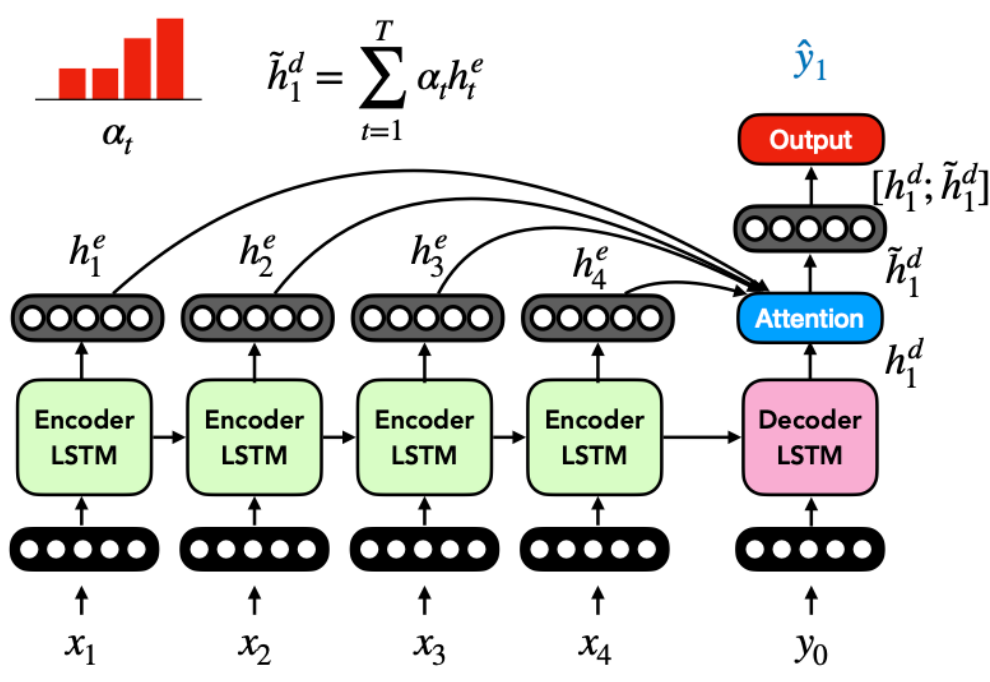
\includegraphics[width=0.36\linewidth]{images/img_20260519_143524.png}
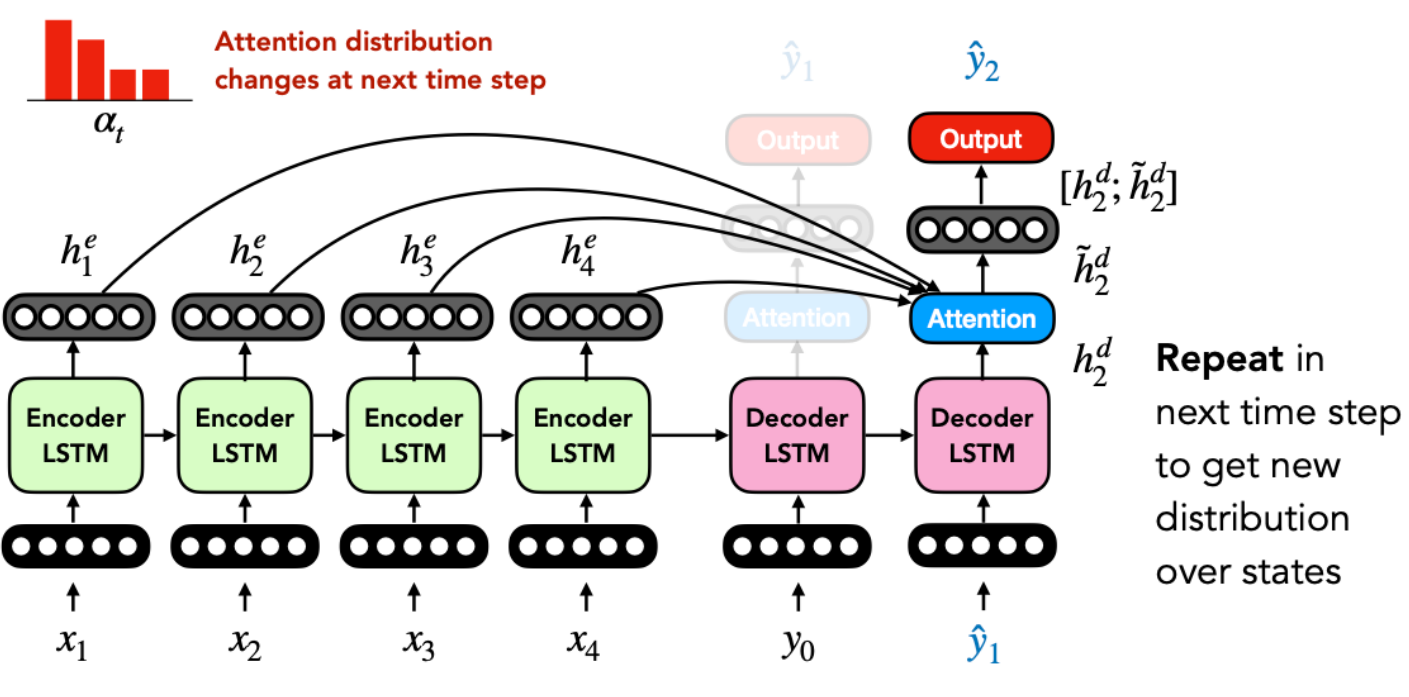
\includegraphics[width=0.5\linewidth]{images/img_20260519_143705.png}
\end{center}

\subsection{Bonus: interpretability}
A nice side benefit of attention is that, by plotting $\alpha_t$ at each generation step,
we can \textbf{visualise} which input words the model looks at when producing each output
word. On a French--English translation task this typically yields a near-diagonal alignment
matrix, with off-diagonal entries appearing exactly where the languages reorder words. We get
\emph{word alignment for free} as a by-product of training.

\begin{center}
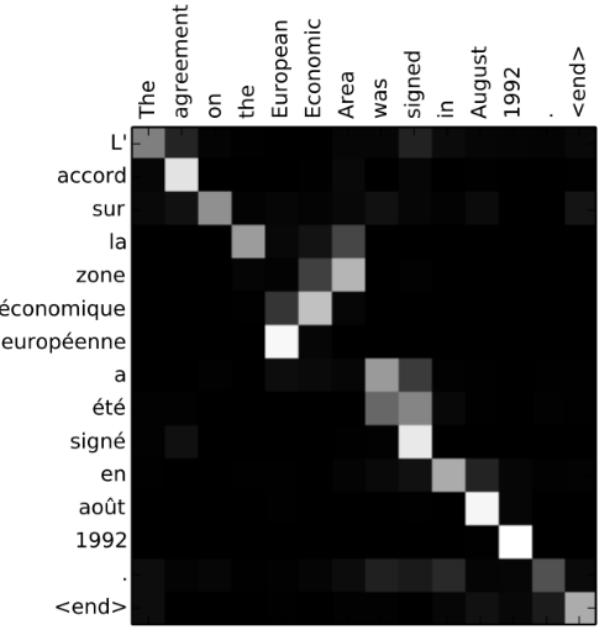
\includegraphics[width=0.35\linewidth]{images/img_20260519_144205.png}
\end{center}

\subsection{Recurrence as problem}
Attention solves the bottleneck problem of RNNs (the decoder can now look at every encoder
state), but the \textbf{encoder itself is still recurrent}: the state $h^{e}_{t}$ depends on
$h^{e}_{t-1}$, so we cannot compute the encoder hidden states in parallel. On modern hardware
(GPUs/TPUs), this is a severe limitation -- we want the model to be \textbf{parallelisable}
across the sequence length. This leads us to transformers.

\section{Transformers}
The \textbf{transformer} removes recurrence altogether and encodes a sequence using only
\textbf{self-attention} and \textbf{feed-forward} layers.
\begin{center}
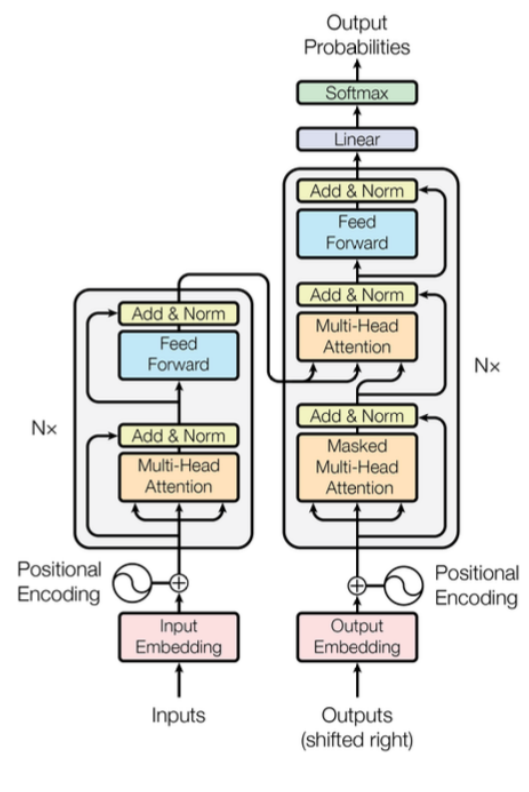
\includegraphics[width=0.38\linewidth]{images/img_20260519_144645.png}
\end{center}

\subsection{Self-attention}
The key idea is to apply attention to the input \emph{within itself}: each token gets to
attend to every other token in the same sequence -- including itself. In the encoder, at
layer $\ell$, every element plays \emph{all three roles}: each token is at once a query, a
key, and a value.

For a single ``query token'' $h^{0}_{s}$ at position $s$, self-attention computes
\begin{center}
  pairwise attention score \quad attention distribution \quad weighted sum 
\end{center}
\[
  \mathbf{a} \;=\; \frac{(\mathbf{W}^{Q} q)\,(\mathbf{W}^{K} K)}{\sqrt{d}},
  \qquad \alpha \;=\; \mathrm{softmax}(\mathbf{a}),
  \qquad \tilde{h}^{\ell}_{s} \;=\; W^{O}\, \alpha\, ( V \mathbf{W}^{V} ),
\]
where:
\begin{itemize}
  \item $q = h^{\ell}_{s}$ is the query (one element of the sequence);
  \item $K = V = \{ h^{\ell}_{t} \}_{t=0}^{T}$ are the keys and values (\emph{all} elements);
  \item $\mathbf{W}^{Q}, \mathbf{W}^{K}, \mathbf{W}^{V}$ are \textbf{learned} projections that turn the same input vector into a query, a key and a value -- they are what makes the three roles different;
  \item $W^{O}$ is a final output projection.
\end{itemize}

\paragraph{The intuition behind queries, keys and values}
A helpful way to picture the three roles is as a question--answer game. Each token uses its
\textbf{query} to \emph{ask a question} about the others: a noun like \emph{creature}, in the
phrase ``a fluffy blue creature'', is effectively asking ``are there any adjectives just before
me?''. Each token uses its \textbf{key} to \emph{answer}: the words \emph{fluffy} and
\emph{blue} produce keys that say ``yes, I am an adjective sitting right before you'', so their
keys \emph{align} with the query of \emph{creature} -- which is exactly why their dot products
(the attention scores) are large. Finally, the \textbf{value} answers a different question:
``if I am relevant to you, what should I add to your meaning?''. In short, the query decides
\emph{what to look for}, the key decides \emph{who matches}, and the value decides \emph{what
gets passed along}.

\paragraph{Queries and keys live in a smaller space}
The query and key projections $\mathbf{W}^{Q}, \mathbf{W}^{K}$ do not preserve the embedding
dimension: they map each embedding (dimension $d \sim 12\,000$ in GPT-3) down to a much smaller
\textbf{query--key space} of dimension $d_{k}$ (typically $d_{k} = 128$). The scores are dot
products computed in this smaller space, and the $d$ appearing in the $\sqrt{d}$ scaling factor
is precisely this query--key dimension $d_{k}$. Working in a low-dimensional query--key space
also keeps the number of attention parameters modest -- which matters a great deal once many
heads are run in parallel.

\vspace{-15pt}
\begin{center}
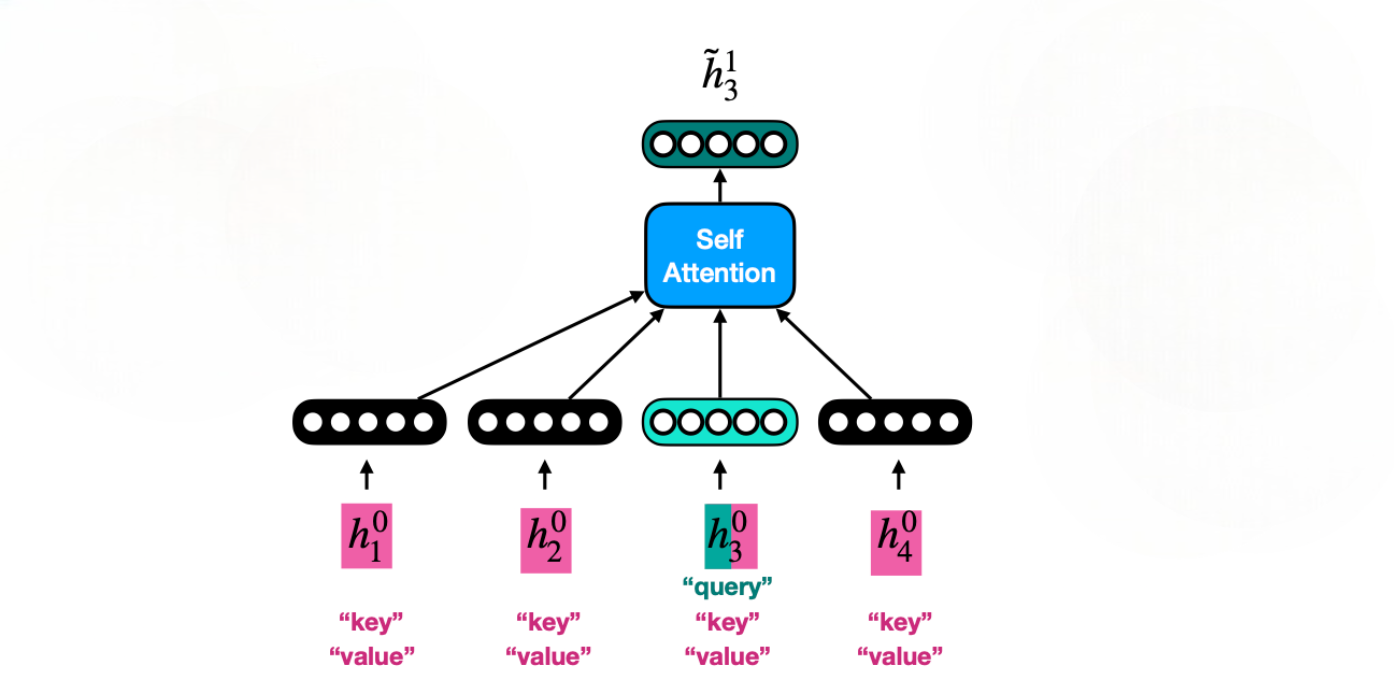
\includegraphics[width=0.92\linewidth]{images/img_20260519_150252.png}
\end{center}

This is repeated with every token playing the role of the query, in parallel, producing one
output vector $\tilde{h}^{\ell}_{s}$ per input position. The whole layer is just a few matrix
multiplications -- there is no recurrence and the computation across positions is fully
parallel.

\begin{center}
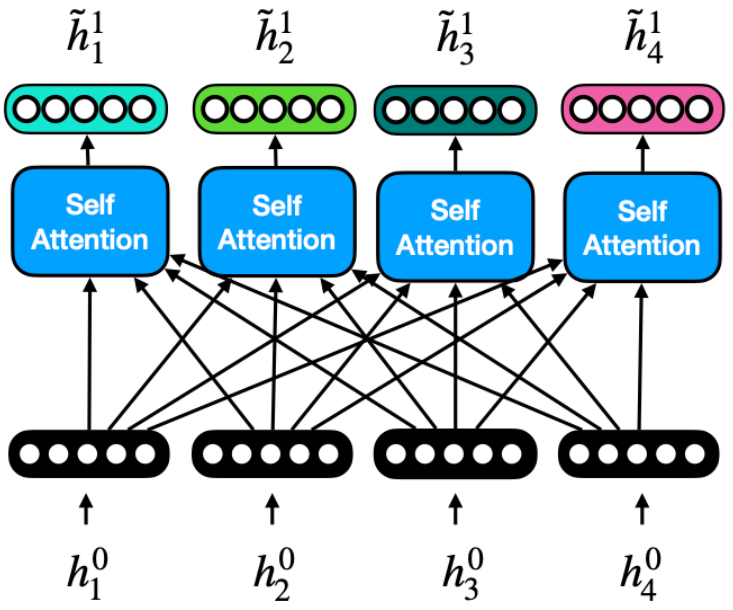
\includegraphics[width=0.45\linewidth]{images/img_20260519_145954.png}
\end{center}

\paragraph{Example walk-through.} Take the sentence ``Nobel committee awards Strickland who
advanced optics''. For each word, $W^{Q}, W^{K}, W^{V}$ produce a query, a key and a value.
\begin{center}  
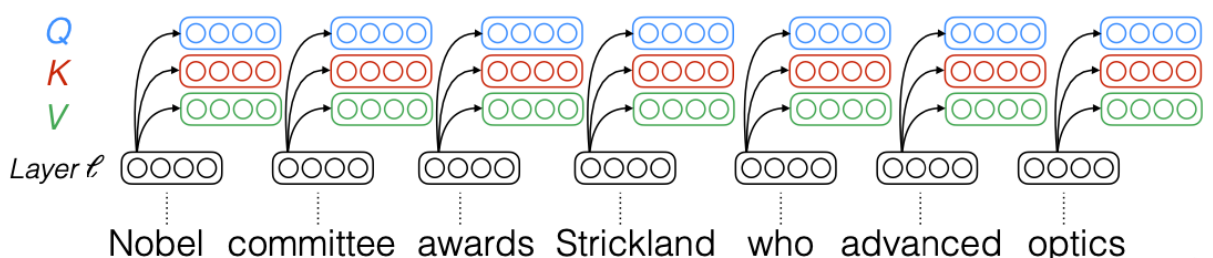
\includegraphics[width=0.8\linewidth]{images/img_20260519_153724.png}
\end{center}

Comparing the query of every word with the keys of all words gives an attention matrix $A$
whose row $s$ encodes \emph{which words token $s$ pays attention to}.

\begin{center}  
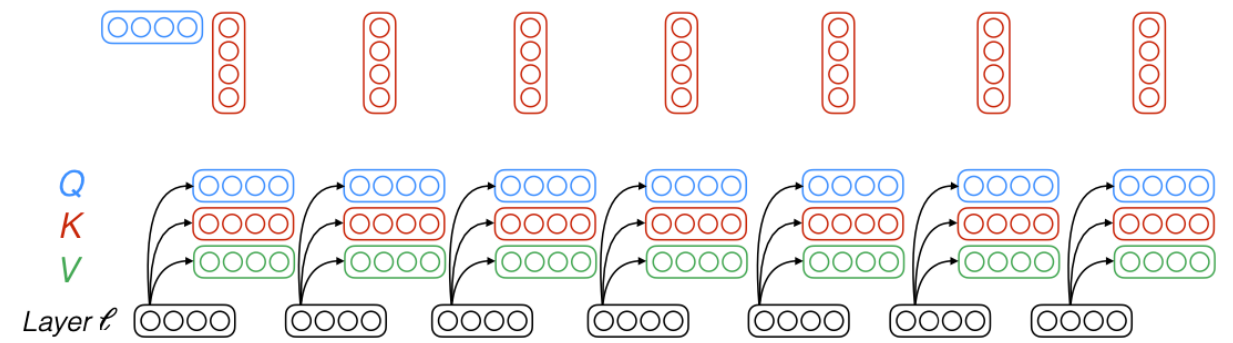
\includegraphics[width=0.8\linewidth]{images/img_20260519_154728.png}
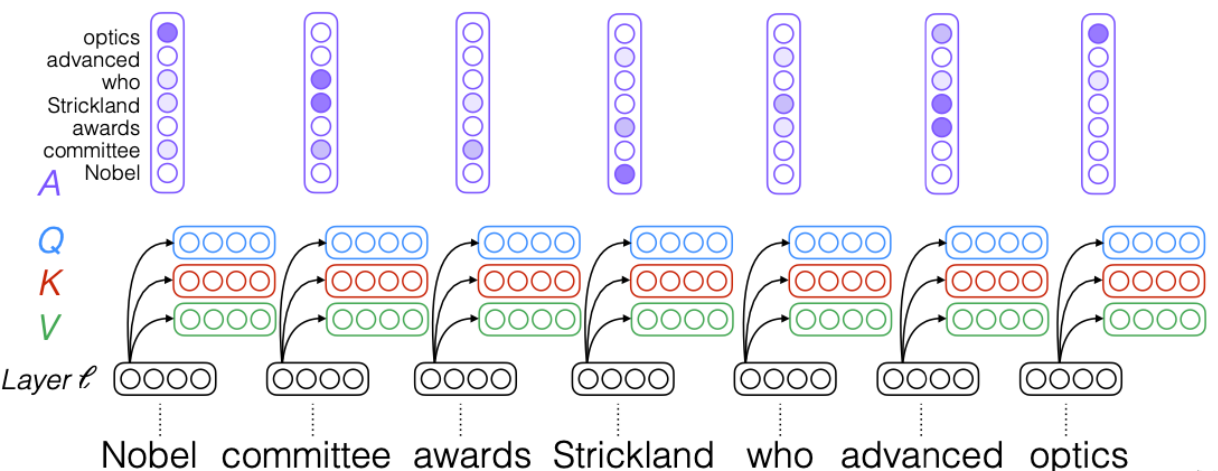
\includegraphics[width=0.8\linewidth]{images/img_20260519_154148.png}
\end{center}

Multiplying $A$ by the
values produces a new representation $M$ of each token, enriched by the rest of the sentence
-- e.g, the representation of ``Strickland'' may now also encode information from
``awards'' and ``optics''.

\begin{center}
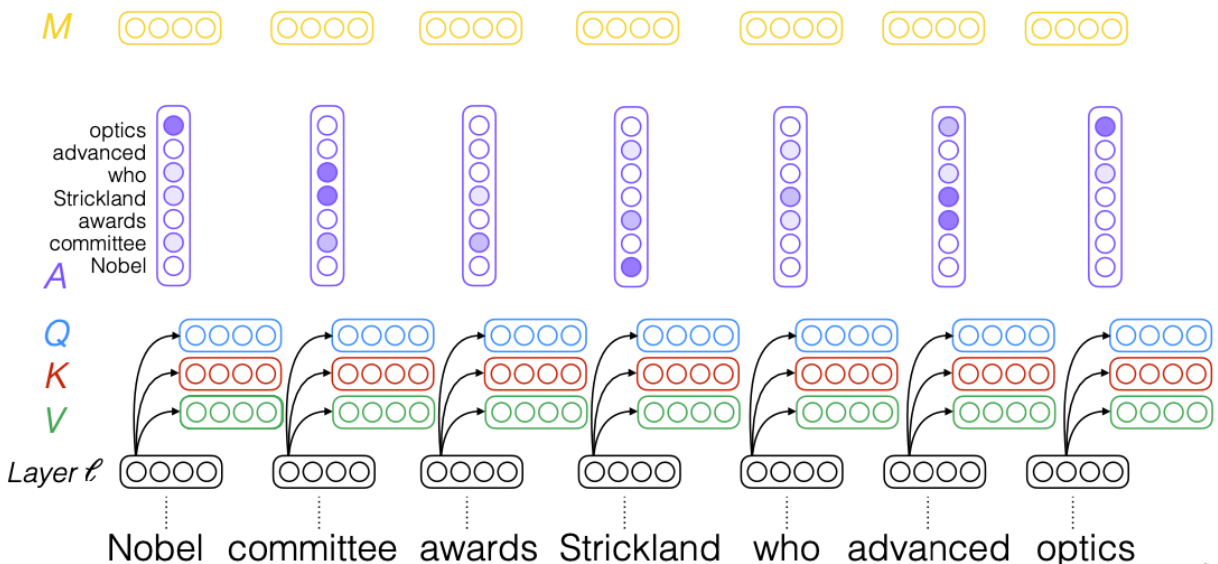
\includegraphics[width=0.8\linewidth]{images/img_20260519_152036.png}
\end{center}

\paragraph{Attention computes an additive update}
It is worth being precise about \emph{how} a token's representation is refined, because it
connects directly to the residual connections. The attention output $\tilde{h}^{\ell}_{s}$ is
best read not as a replacement but as a \textbf{proposed change} $\Delta e$: the value vector of
a relevant word answers ``here is what I should add to your embedding'', and the weighted sum of
these value vectors (weighted by the attention scores $\alpha$) is the change to apply. Through
the residual connection, this change is then \emph{added} to the original, context-free
embedding,
\[
  e_{\text{new}} \;=\; e + \Delta e, \qquad \Delta e \;=\; \tilde{h}^{\ell}_{s},
\]
so each token keeps what it already encoded and attention only \emph{nudges} it towards a more
context-specific direction -- exactly the $x + \mathrm{sublayer}(x)$ logic.

For the example \textit{"a fluffy blue creature"}, the
embedding of \emph{creature} starts generic, and attention adds a ``fluffiness'' and
``blueness'' component until it points towards \emph{fluffy blue creature}.

\subsection{Multi-head self-attention}
A single attention pattern is restrictive: a word may need to attend to its grammatical
subject \emph{and} to a related noun \emph{and} to a pronoun, all at once. \textbf{Multi-head
self-attention} runs $H$ independent self-attention computations (``heads'') in parallel,
each with its own $\mathbf{W}^{Q}_{h}, \mathbf{W}^{K}_{h}, \mathbf{W}^{V}_{h}$. The outputs
$M_{1}, \dots, M_{H}$ are concatenated and projected back to the original dimension. Each
head can specialise in a different type of relation.

\begin{center}
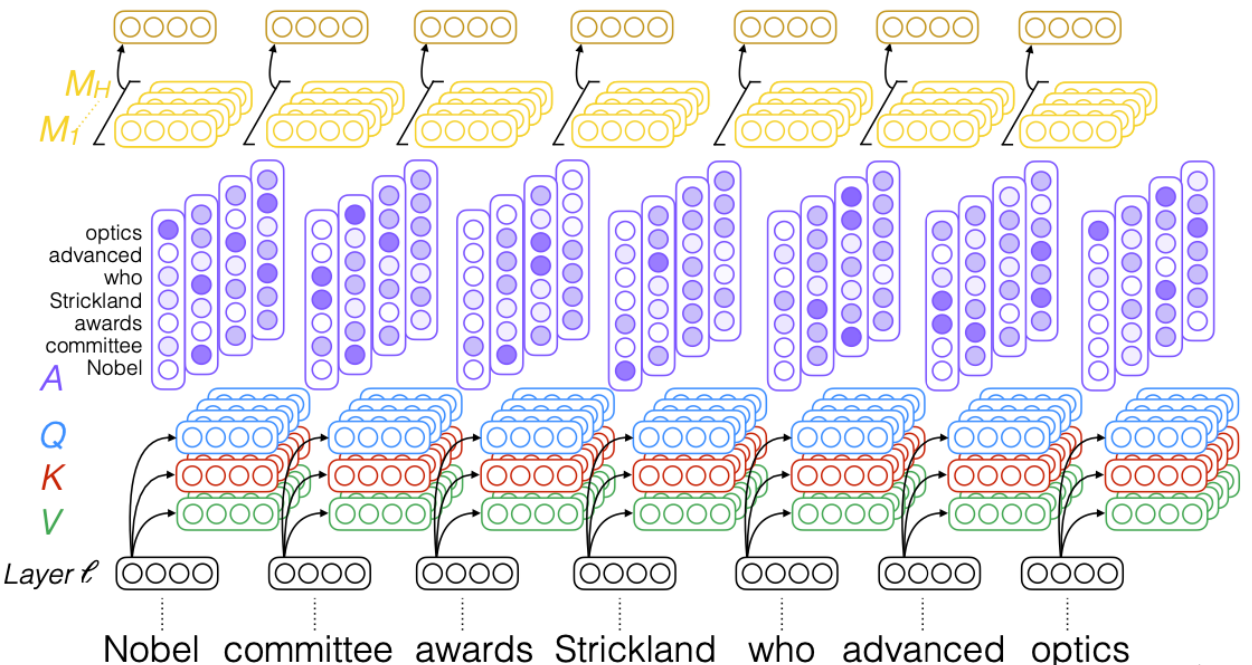
\includegraphics[width=0.8\linewidth]{images/img_20260519_153305.png}
\end{center}

This is \emph{the main innovation of the transformer}.

\subsection{The transformer block}

\begin{wrapfigure}{r}{0.2\linewidth}
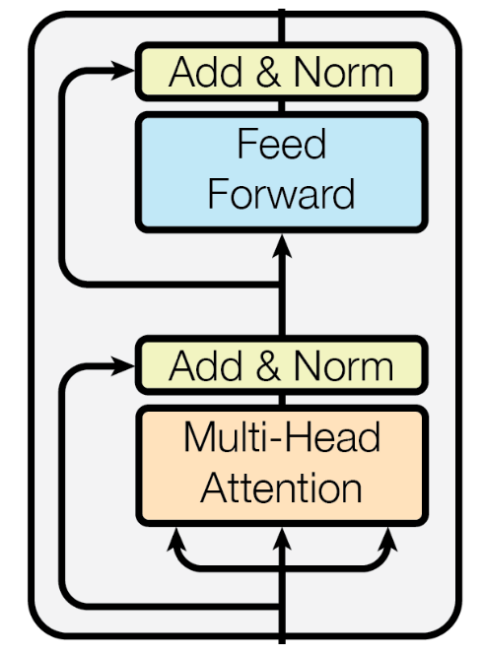
\includegraphics[width=\linewidth]{images/img_20260519_153513.png}
\end{wrapfigure}

Multi-head attention is the heart of a transformer block, but a block contains more:
\begin{itemize}
  \item a \textbf{multi-head self-attention} layer;
  \item a \textbf{feed-forward network} (a small MLP applied independently at each position);
  \item \textbf{residual connections} around each sub-layer ($x + \mathrm{sublayer}(x)$);
  \item \textbf{layer normalisations} after each residual.
\end{itemize}
\clearpage
\paragraph{What the feed-forward sub-layer does}
Whereas the attention sub-layer is where the vectors \emph{exchange} information, in the
feed-forward sub-layer they do \textbf{not} talk to each other at all: the same small MLP is
applied independently at every position. A useful intuition is to picture it as asking a long
list of questions about each vector -- ``does this encode a noun?'', ``something royal?'',
``a past-tense verb?'', \dots\ -- and updating the vector according to the answers. This is
widely believed to be where much of the model's stored factual and relational knowledge lives.
The two sub-layers thus play complementary roles: \emph{attention moves information between
tokens, the feed-forward layer processes each token in place}, and alternating them is what
builds up rich representations.

\subsection{Full transformer}
\begin{wrapfigure}{r}{0.3\linewidth}
\vspace{-65pt}
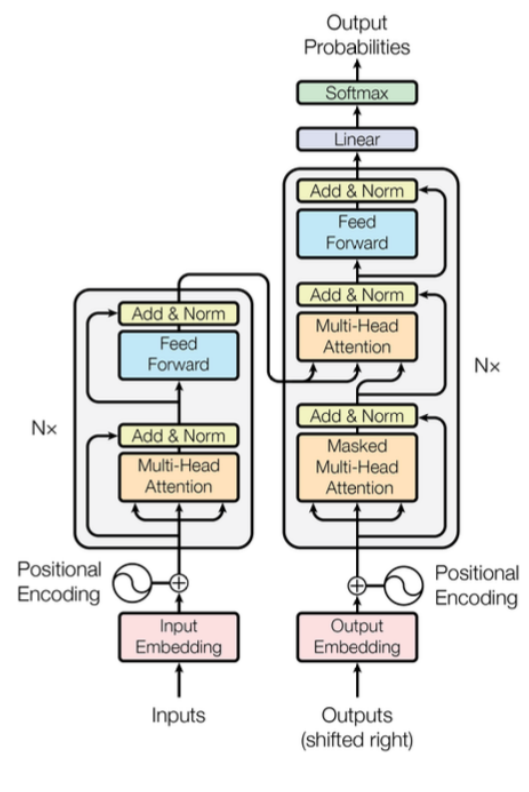
\includegraphics[width=\linewidth]{images/img_20260519_144645.png}
\end{wrapfigure}

The full transformer encoder is multiple cascaded transformer blocks; each block refines the representations and
builds up increasingly compositional features of the input.

The transformer decoder (right side) is similar to encoder, but each blocks contains \emph{two} attention
sub-layers:
\begin{itemize}
  \item First layer of block is \textbf{masked} multi-headed attention
  \item Second layer is multi-headed attention over \textit{final-layer} encoder outputs \textbf{(cross-attention)}
  \item The third layer is feed-forward network (as encoder).
\end{itemize}

\subsection{The decoder side: masked self-attention and cross-attention}
\subsubsection{Masked self-attention}
The decoder generates tokens one at a time, so when producing token $t$ it must only see
tokens $< t$ -- otherwise, at training time, it could trivially cheat by looking at the answer.

Masked self-attention enforces this by setting the attention scores of future
positions to $-\infty$ before the softmax, which makes the corresponding weights $\alpha = 0$:
\[
  a_{st} \;=\; \frac{(\mathbf{W}^{Q} h^{\ell}_{s})^{T}\,(\mathbf{W}^{K} h^{\ell}_{t})}{\sqrt{d}},
  \qquad
  a_{st} \;:=\; a_{st} - \infty \quad \text{for } s < t,
  \qquad
  \alpha_{st} \;=\; \frac{e^{a_{st}}}{\sum_{j} e^{a_{sj}}} \;=\; 0 \text{ for } s < t.
\]

\begin{center}
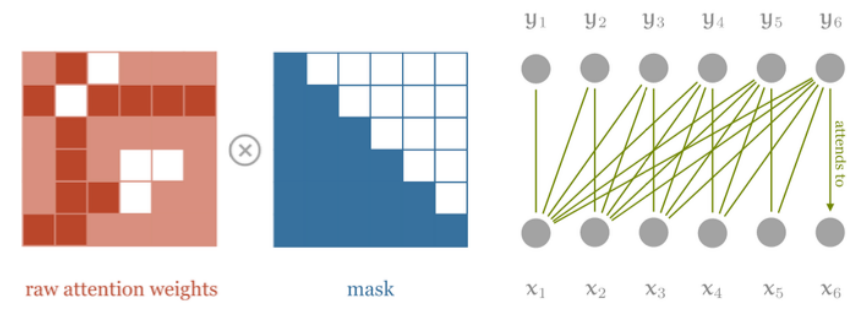
\includegraphics[width=0.6\linewidth]{images/img_20260519_163609.png}
\end{center}
This mask is applied as soon as the model as to respect a causal structure, i.e., when position $t$ 
must see only the positions $\leq t$. So when generating token by token (e.g., decoder used to generate text)

\paragraph{Why this would be cheating: how the decoder is trained}
The reason the model \emph{could} cheat is that training does not proceed the same way as
generation. At generation time the decoder produces one token at a time, so to predict token
$t$ it only \emph{has} tokens $1, \dots, t-1$ -- the future does not exist yet, and there is
nothing to peek at. Training, however, uses an efficiency trick: instead of running $T$
separate forward passes for a target of length $T$, we feed the \textbf{entire target sequence
at once} (using the ground-truth tokens as inputs -- so-called \emph{teacher forcing}) and ask
\emph{every} position to predict the token that follows it, in a single forward pass. One
training example then yields $T$ signals at once: position $1$ predicts $y_{1}$, position $2$
predicts $y_{2}$, and so on.

The catch is that this puts the \emph{whole} target sequence into the input. Since
self-attention lets every position attend to every other, position $t$ could simply look ahead
at position $t+1$ -- which already contains the answer $y_{t}$ -- and copy it, reducing
``predict the next token'' to the trivial ``read the next slot''. Masking the future before the
softmax removes exactly these forward-looking entries, so each position sees only its past:
training conditions then match generation conditions, while the parallel-training speed-up is
preserved (still a single forward pass, just with the forbidden future entries of the
attention matrix set to zero).
\vspace{-8pt}
\paragraph{Example} For a translation task ``Le chat dort'' $\to$ ``The cat sleeps'', we build
two sequences shifted by one position:
\[
\begin{array}{l|cccc}
\text{position } t & 1 & 2 & 3 & 4 \\ \hline
\text{decoder input} & \texttt{<start>} & \text{The} & \text{cat} & \text{sleeps} \\
\text{target } y_{t} & \text{The} & \text{cat} & \text{sleeps} & \texttt{<end>}
\end{array}
\]
with decoder input = outputs (shifted right) in the image

At each position $t$, the decoder must predict $y_{t}$ using only the inputs at positions
$1, \dots, t$. Without masking, when processing position $t = 1$ the decoder could attend to
position $t = 2$ of its input, which contains exactly the target $y_{1} = \text{``The''}$ --
the model would learn the trivial shortcut of copying the next input token and collapse at test time. 
Masking the future before the softmax prevents this.

\subsubsection{Cross-attention}
\begin{wrapfigure}{r}{0.3\linewidth}
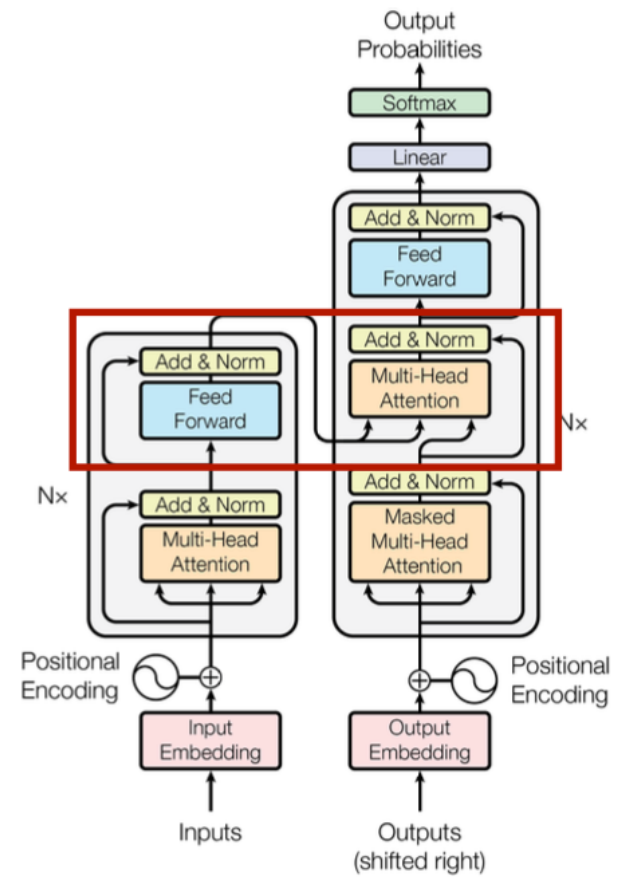
\includegraphics[width=\linewidth]{images/img_20260519_165104.png}
\end{wrapfigure}

This is the same classical attention mechanism that we saw in the RNN encoder--decoder model:
the decoder uses its current state as a \textbf{query} to attend over the \textbf{final}
encoder layer's outputs (which act as keys and values). This is what lets the decoder
\emph{look at the source sentence} when translating.

So in a decoder block we have, in order: masked self-attention $\to$ cross-attention $\to$
feed-forward, each followed by Add\,\&\,Norm.
\vspace{-8pt}
\paragraph{Example} Consider translating ``Le chat dort'' $\to$ ``The cat sleeps''.
\begin{enumerate}
  \item The encoder reads ``Le chat dort'' and produces three output vectors
        $h^{e}_{1}, h^{e}_{2}, h^{e}_{3}$, one per French token.
  \item The decoder has so far produced \texttt{<start>}, ``The'', and is about to predict
        the next token. Inside the corresponding decoder block:
        \begin{itemize}
          \item \textbf{Masked self-attention} mixes information across the English tokens
                already generated (\texttt{<start>}, ``The'') -- English speaking to English.
          \item \textbf{Cross-attention} uses the current decoder state as a query to look
                at the three French vectors. Its query will most likely match the key of
                ``chat'' $\Rightarrow$ high attention on ``chat'' $\Rightarrow$ the value of
                ``chat'' is pulled into the decoder's representation. The decoder now knows
                that the word to produce is related to ``chat''.
        \end{itemize}
  \item The feed-forward sub-layer refines the representation, and the output softmax
        predicts ``cat''.
\end{enumerate}

\subsection{Position embeddings}
A self-attention layer is, by construction, \textbf{permutation-equivariant}: it does not see
the order of its inputs (it only sees a \emph{set} of vectors). For language this is
obviously wrong -- ``dog bites man'' $\neq$ ``man bites dog''. We therefore add a
\textbf{position embedding} $p_{i}$ to each input embedding to inject positional information.

\begin{center}  
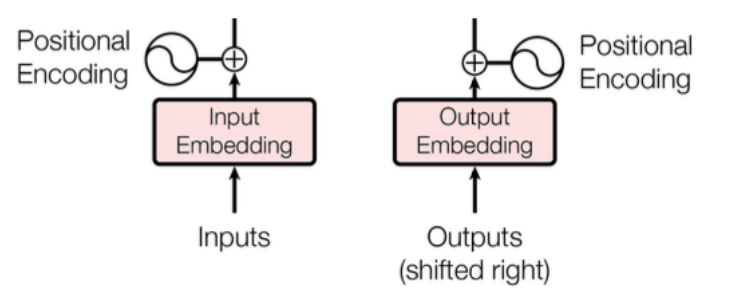
\includegraphics[width=0.55\linewidth]{images/img_20260519_170508.png}
\end{center}

The original transformer used a sinusoidal encoding:
\[
  p_{i} \;=\; \begin{pmatrix}
    \sin(i/10000^{2 \cdot 1/d}) \\
    \cos(i/10000^{2 \cdot 1/d}) \\
    \vdots \\
    \sin(i/10000^{2 \cdot \frac{d}{2}/d}) \\
    \cos(i/10000^{2 \cdot \frac{d}{2}/d}) \\
  \end{pmatrix},
\]
which gives every position a distinct, smoothly-varying signature.

\textbf{In practice}, learned position embeddings (a simple lookup table $p_{i}$ for each
position $i$, trained end-to-end with the rest of the model) work just as well and are now
standard.

\begin{center}
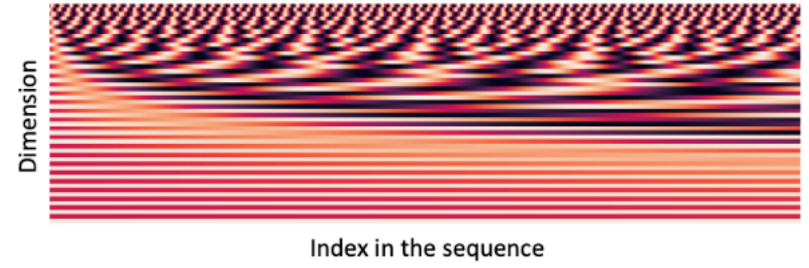
\includegraphics[width=0.6\linewidth]{images/img_20260519_170527.png}
\end{center}

\section{GPT: a decoder-only transformer}
\begin{wrapfigure}{r}{0.3\linewidth} 
\vspace{-30pt}
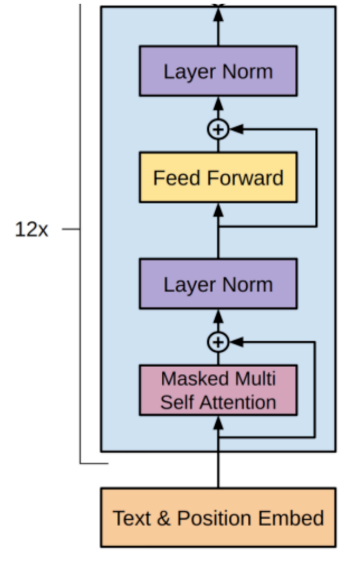
\includegraphics[width=\linewidth]{images/img_20260519_171153.png} 
\end{wrapfigure}

\textbf{GPT} (Generative Pretrained Transformer) is called a \emph{decoder} transformer
because its job is to generate text autoregressively. Its block, however, \emph{mixes
features} from the encoder and decoder of the original transformer:
\begin{itemize}
  \item from the \textbf{decoder}, it inherits the \textbf{masked multi-head self-attention}
        (so the model never sees future tokens during training);
  \item from the \textbf{encoder}, it inherits the simple two-sublayer structure
        (multi-head attention $\to$ feed-forward), with the usual residual connections and
        layer norms. There is \textbf{no cross-attention}: there is no encoder for the
        decoder to attend to, so each block just does self-attention over its own past.
\end{itemize}

\subsection{(Pre)Training}
GPT is pretrained on a large corpus of raw text (originally TorontoBooks, $\sim$13~GB, 7000
unpublished books) split into windows of 512 tokens. Its training objective is
\textbf{next-word prediction} (language modelling):
\[
  \mathcal{L} \;=\; \sum_{t} -\log P\big( y_{t} \;|\; y_{1}, \dots, y_{t-1} \big).
\]
The model is purely self-supervised -- the supervision is the next token of the text itself.

\paragraph{From the final vector to a distribution: unembedding, logits and temperature}
How is the distribution $P(\,\cdot \mid y_{1}, \dots, y_{t-1})$ actually produced? Once the
input has flowed through all the blocks, we take the final vector of the sequence and apply a
learned \textbf{unembedding matrix} $W_{U}$. It has one row per vocabulary token (so it is
essentially the embedding matrix $W_{E}$ with its dimensions swapped) and maps the final
vector to a list of $|V|$ real numbers -- one raw score per possible next token. These
unnormalised scores are called the \textbf{logits}. They can be negative or larger than $1$
and need not sum to $1$, so we pass them through a \textbf{softmax} to obtain a valid
distribution:
\[
  P(\text{next token} = i) \;=\; \frac{e^{z_{i}/T}}{\sum_{j} e^{z_{j}/T}},
\]
where $z_{i}$ are the logits and $T$ is a \textbf{temperature} constant. A large $T$ flattens
the distribution (more uniform, hence more ``creative'' samples); a small $T$ sharpens it so
the largest logit dominates; and $T \to 0$ recovers the deterministic \emph{argmax}, i.e.\
always picking the single most likely token. At training time this read-off is done at
\emph{every} position simultaneously -- each final vector predicts the token that should follow
it, which is exactly the sum over $t$ in the loss above; at generation time we only need the
score from the last position.

\paragraph{Generating text}
Once we can produce a distribution over the next token, generation is just a loop -- exactly
the autoregressive idea seen for RNNs: start from a seed prompt, \textbf{sample} a token from
the predicted distribution, \textbf{append} it to the sequence, and feed the whole thing back
in to predict the next one, repeating until an end-of-sequence token. Sampling (rather than
always taking the argmax) is where the temperature above comes into play.

A \textbf{chatbot} is built directly on top of this: one prepends a \textbf{system prompt} that sets up a helpful
assistant, feeds the user's message as the start of the dialogue, and lets the model predict
what such an assistant ``would say next'' (the extra fine-tuning step discussed below is what
makes this behave well).

\textbf{Remark.} The model can only attend over a fixed number of tokens at once -- its
\textbf{context size} (the $512$-token window above). This is why a very long conversation can
make a model appear to ``lose the thread'': content that falls outside the context window is
simply no longer visible to it.

\subsubsection{From input to output: assembling the blocks}
We can now assemble all the pieces into the complete journey of a piece of text through a
GPT-style transformer, from raw input to a next-token distribution:
\begin{enumerate}
  \item \textbf{Tokenise and embed}: split the text into tokens, look each up in the embedding
        matrix $W_{E}$ to get a sequence of vectors, and add a \textbf{position embedding} to
        each.
  \item \textbf{Stack of $N$ identical blocks}: each block refines the vectors with, in order,
        a \textbf{masked multi-head self-attention} sub-layer (tokens exchange information,
        each looking only at the past) followed by a \textbf{feed-forward} sub-layer (each
        vector processed in place), every sub-layer wrapped in a residual connection and a
        layer norm. Across the stack, every vector gradually soaks up context.
  \item \textbf{Unembed}: multiply the final vector by $W_{U}$ to obtain the \textbf{logits},
        one score per vocabulary token.
  \item \textbf{Softmax (with temperature)} turns the logits into a probability distribution
        over the next token.
  \item \textbf{Generate}: sample a token, append it, and loop back to step~1.
\end{enumerate}
The two workhorses are therefore \textbf{multi-head attention}, which moves information
\emph{between} tokens, and the \textbf{feed-forward} layer, which computes \emph{within} each
token; everything else -- embeddings, position encodings, residuals, layer norms, unembedding
and softmax -- is the wiring that turns these two operations into a model mapping text to a
distribution over what comes next.

\subsection{Fine-tuning and the paradigm shift}
After pretraining, GPT can be \textbf{fine-tuned} on individual downstream tasks
(classification, entailment, similarity, multiple-choice question answering) by appending a
small task-specific head and continuing to train on the new dataset. The pretrained weights
serve as initialization.
\begin{center}
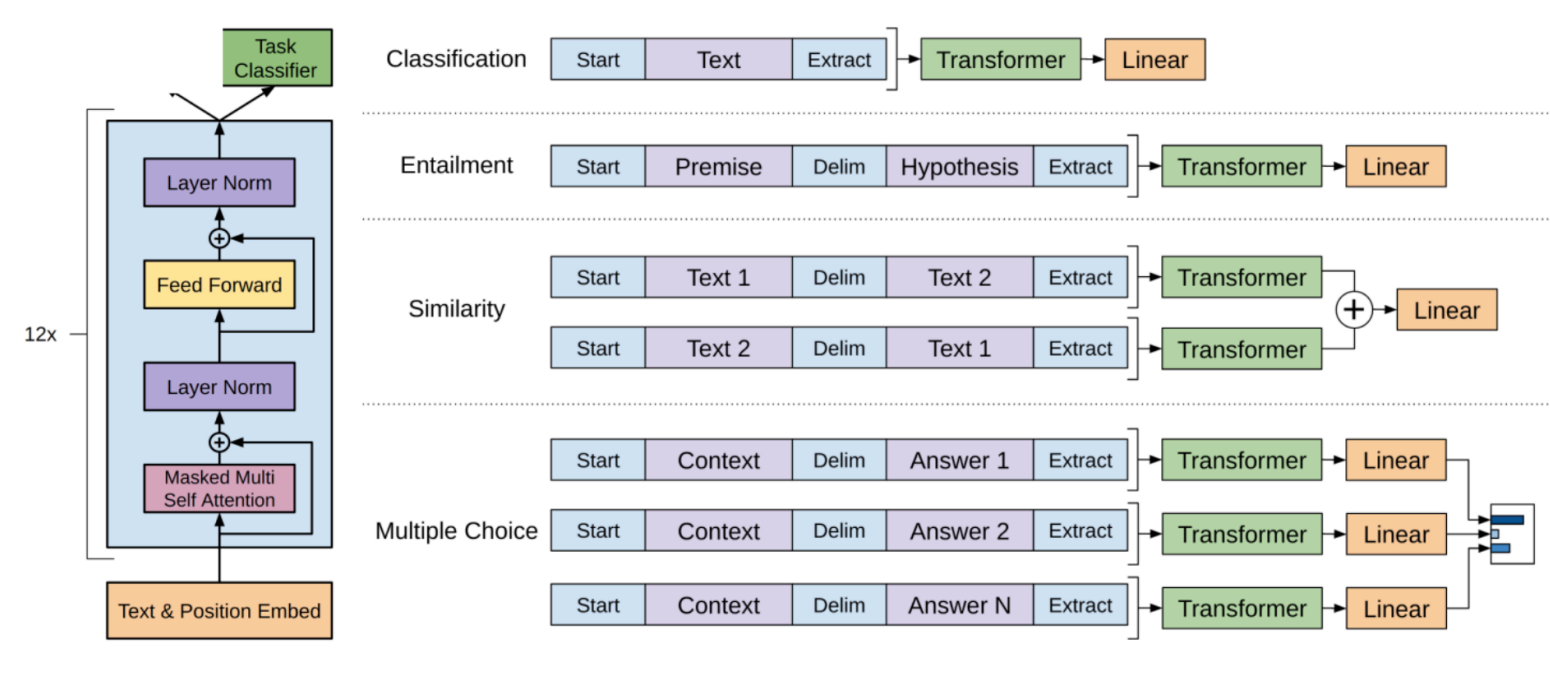
\includegraphics[width=0.9\linewidth]{images/img_20260519_172629.png}
\end{center}

This represents a fundamental \textbf{paradigm shift} in NLP:
\begin{itemize}
  \item \emph{Before}: pretrain only the \textbf{word embeddings} (Word2Vec, GloVe,
        fastText), then train a task-specific model from scratch on top of them.
  \item \emph{After}: pretrain a \textbf{full model} (millions to billions of parameters),
        and reuse it almost as-is for many downstream tasks.
\end{itemize}

\subsection{Scale}
The history of GPT is largely a history of scaling up:
\begin{itemize}
  \item GPT (2018): 117M parameters, trained on 13GB of data $\sim$1B tokens
  \item GPT-2 (2019): 1.5B parameters, trained on $\sim$40\,GB of data;
  \item GPT-3 (2020): 175B parameters, $\sim$500GB data $\sim$300B tokens;
  \item GPT-4 (2023): rumoured $\sim$1.76T parameters, $\sim$13T tokens.
\end{itemize}
Each step came with qualitatively new capabilities, often summarised under the umbrella of
``emergent abilities''.

\subsection{Other famous text models}
GPT is the most well-known but not the only transformer-based language model:
\textbf{BERT} (Devlin et al., 2018), \textbf{RoBERTa} (Liu et al., 2019),
\textbf{DistilBERT} (Sanh et al., 2019), \textbf{Electra} (Clark et al., 2020), and at EPFL,
\textbf{Meditron} (medical LLM) and \textbf{Apertus} (fully open multilingual LLM).

\textbf{Remark.} BERT-style models are \emph{encoder-only} transformers, pretrained with a
\textbf{masked language modelling} objective (predict a random subset of masked-out tokens
using the entire surrounding context, not just the past). They are especially good at
\emph{understanding} tasks, whereas GPT-style decoder-only models are designed for
\emph{generation}.

\section{Transformers beyond text}
Although transformers were developed for NLP applications, transformers (and the attention mechanism) is generic: it
just needs a sequence of vectors as input. The main idea generalizes to other modalities.

\subsection{Transformers for images}
The most direct approach is to flatten an image into a sequence of pixel vectors and feed
them to a standard transformer (Chen et al., 2020, \emph{Generative Pretraining from Pixels}).

\begin{center}
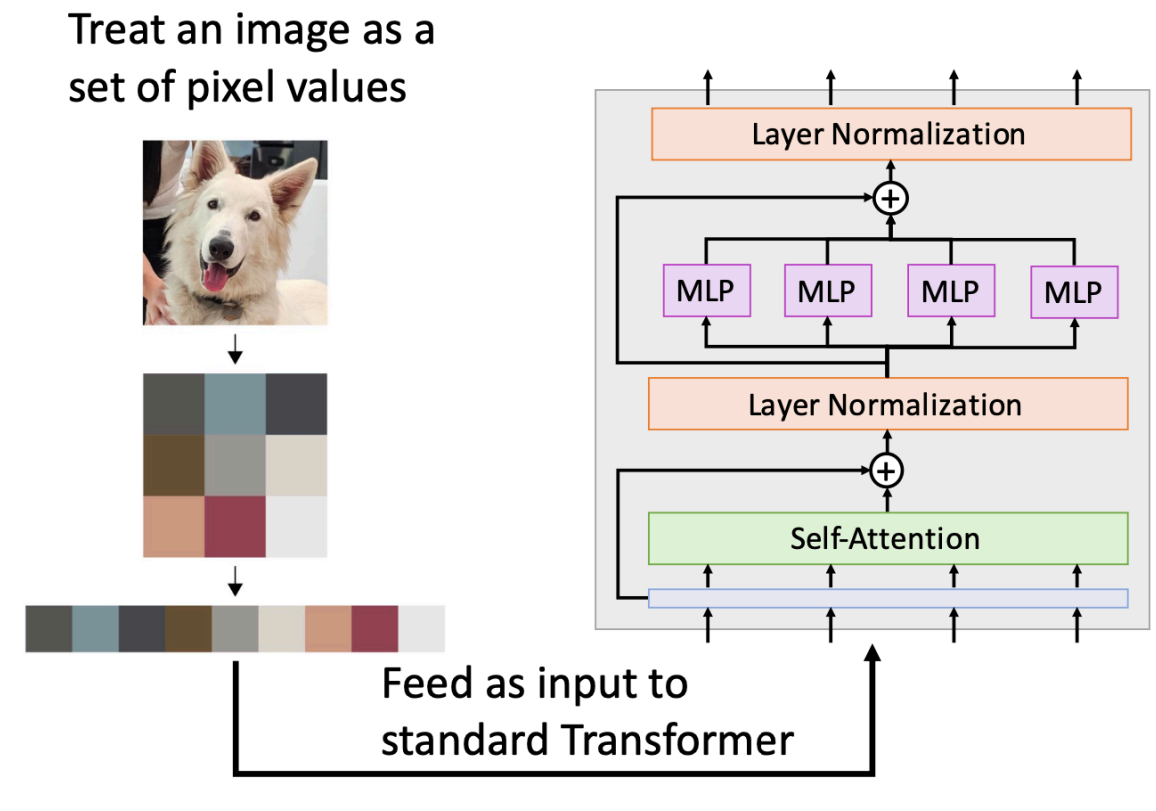
\includegraphics[width=0.7\linewidth]{images/img_20260519_183607.png}
\end{center}

The problem is \textbf{memory}: self-attention on $N$ tokens needs $O(N^{2})$ memory for the
attention matrix, and an $R \times R$ image gives $N = R^{2}$ tokens, hence $R^{4}$ entries
per attention matrix per head per layer. The slide quotes 768~GB for a single example at
$R = 128$ with 48 layers and 16 heads -- clearly impractical.
\clearpage
\subsection{Vision Transformer (ViT)}
\textbf{Vision Transformer} (Dosovitskiy et al., 2021, ``An Image is Worth $16 \times 16$
Words'') solves this by treating an image not as a set of pixels but as a set of
\textbf{patches}, typically $16 \times 16$ each.

\begin{center}
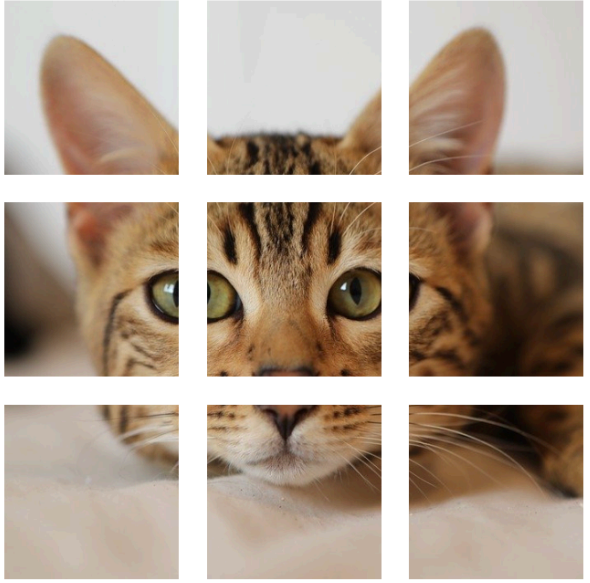
\includegraphics[width=0.4\linewidth]{images/img_20260519_184105.png}
\end{center}An image is split into $N$ non-overlapping
patches, each patch is flattened and projected linearly to a $D$-dimensional vector, and a
\textbf{learned positional embedding} is added. The result is a sequence of $N$ vectors --
exactly the input format expected by a standard NLP transformer.

\begin{center}
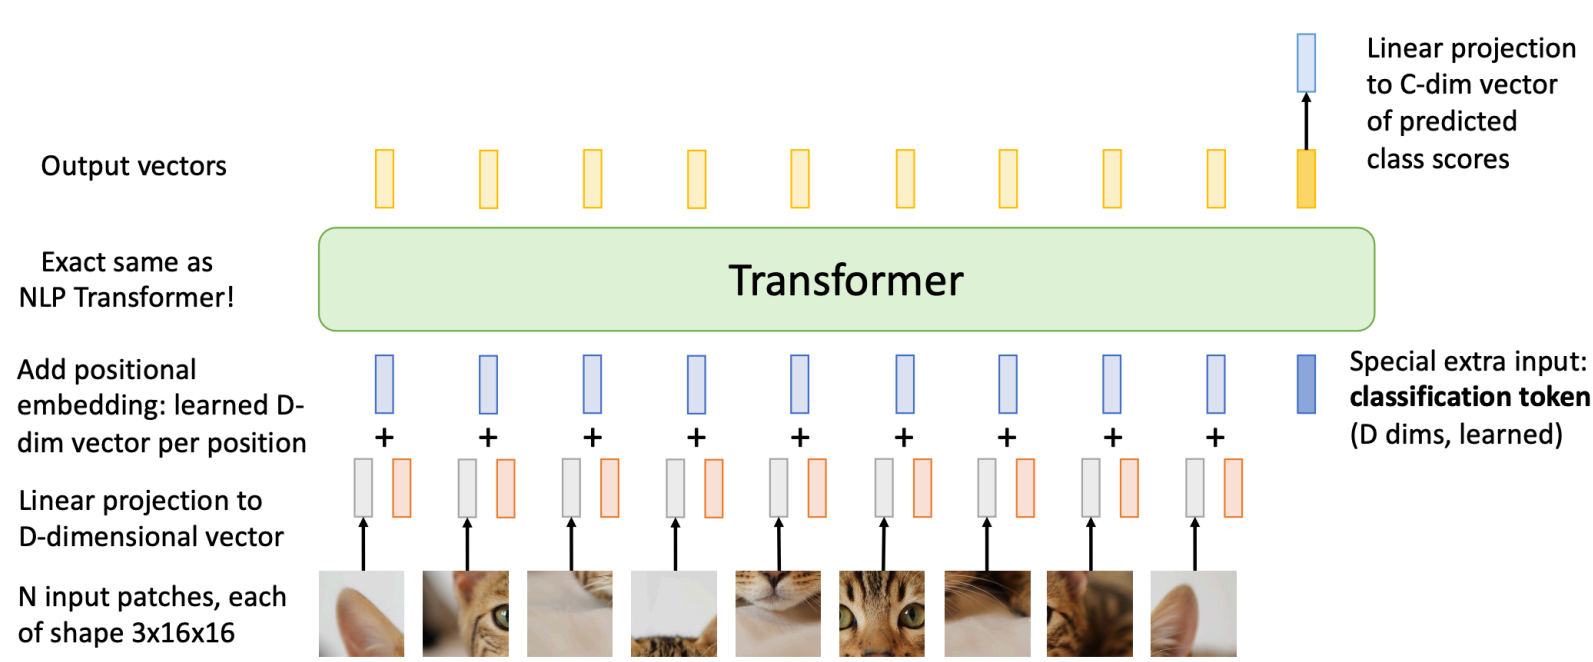
\includegraphics[width=0.9\linewidth]{images/img_20260519_184338.png}
\end{center}

For classification, a special \textbf{classification token} (a learned $D$-dimensional vector)
is prepended to the patch sequence. After the transformer, the output corresponding to that
token is fed to a linear classifier to produce class scores. This is analogous to BERT's
\texttt{[CLS]} token.

\textbf{Two amusing caveats.} ViT is often described as a ``computer vision model without
convolutions'', but:
\begin{itemize}
  \item the very first operation (splitting the image into $p \times p$ patches and
        projecting each to a $D$-vector) is exactly a \texttt{Conv2D} with kernel size $p$
        and stride $p$ -- a convolution;
  \item the position-wise MLPs inside transformer blocks are equivalent to stacks of
        $1 \times 1$ convolutions.
\end{itemize}
So strictly speaking ViT is a network of $p \times p$ and $1 \times 1$ convolutions, plus
self-attention -- but the \emph{spirit} of the architecture is genuinely non-convolutional:
no large spatial kernels, no spatial pooling, no hand-designed hierarchy.

\textbf{Takeaway.} The success of transformers across very different modalities (text, images,
audio, video, proteins, \dots) is one of the strongest empirical arguments that attention is
a remarkably general architectural primitive.

\clearpage
